\documentclass[11pt]{scrartcl}
\usepackage{ucs}
\usepackage[utf8x]{inputenc}
\usepackage[T1]{fontenc}
\usepackage[ngerman,english]{babel} %Text in deutscher Sprache
%\usepackage[english]{babel} %Text in deutscher Sprache
\usepackage{amsmath,amssymb,amstext} %Package für mathematische Umgebung
\usepackage{graphicx} %Bilder hinzufügen
%\usepackage[parfill]{parskip} %no indent as package, else put \noindent
\usepackage{caption}
\usepackage{subcaption}
\usepackage{float}
 
% itemize in coloumns 
\usepackage{etoolbox,refcount}
\usepackage{multicol}

\newcounter{countitems}
\newcounter{nextitemizecount}
\newcommand{\setupcountitems}{%
  \stepcounter{nextitemizecount}%
  \setcounter{countitems}{0}%
  \preto\item{\stepcounter{countitems}}%
}
\makeatletter
\newcommand{\computecountitems}{%
  \edef\@currentlabel{\number\c@countitems}%
  \label{countitems@\number\numexpr\value{nextitemizecount}-1\relax}%
}
\newcommand{\nextitemizecount}{%
  \getrefnumber{countitems@\number\c@nextitemizecount}%
}
\newcommand{\previtemizecount}{%
  \getrefnumber{countitems@\number\numexpr\value{nextitemizecount}-1\relax}%
}
\makeatother    
\newenvironment{AutoMultiColItemize}{%
\ifnumcomp{\nextitemizecount}{>}{3}{\begin{multicols}{2}}{}%
\setupcountitems\begin{itemize}}%
{\end{itemize}%
\unskip\computecountitems\ifnumcomp{\previtemizecount}{>}{3}{\end{multicols}}{}}



\title{Bachelorthesis}
\author{Meikee Pagsinohin}

\begin{document}

\section{Introduction}

	\subsection{Motivation}
		Goal of this project is the improvement in the distinction process between $t\overline{t}\gamma$ and $t\overline{t}$ events in the signal region. Depending on the success, the results can be further used for other projects, which would improve the simulations and their predictions regarding the standard model (SM) and beyond standard model (BSM). 

	\subsection{Approach}
	\label{sec:approach}
		An attempt was perfomed through a multivariate analysis and by developing and training models. At the beginning different variables were analysed and compared and the most promising were used for training. Type of models, denoted MVA in the following, used are boosted decision tree (BDT) and mutilayer perceptron (MLP). The results of the MVAs for three different variable categories were created and in the course of this project analysed and presented.

\section{Background information}
	\subsection{ATLAS detector and data}
	The ATLAS detector is part of the Large Hadron Collider, a particle accelerator, which was built by the research organisation CERN in Genf, Siwtzerland. LHC has a circumference of 27km and is up to 175m deep. Besides ATLAS, there are other experiments as well, such as CMS, ALICE, LHCb. ATLAS can be described by three sub-detectors. All detectors surround the beam pipe, where the particles are accelerated and collided against eachother.
	
	In Figure \ref{fig:detectorsystem}, a sketch of the detectorsystem can be seen. The inner detecor is a tracking chamber for charged partices. It is surrounded by a superconducting solenoid with a magnetic field of 2T used to divert the particle trajectory to measure the momentum. The calorimeter is made up of alternating layers. One is a dense absorber material, which is used to prompt electromagnetic and hadronic showers (ECAL, HCAL). The other layer is of active material used for energy measurement. The muon spectrometer (MS) is positioned in the outermost layer since muons may pass inner layers as well as the calorimeters. It is surrounded by a magnetic field and the diversion is measured by a multiple layer of high precision tracking chambers. 
	
	\begin{figure}[H]
	\centering
	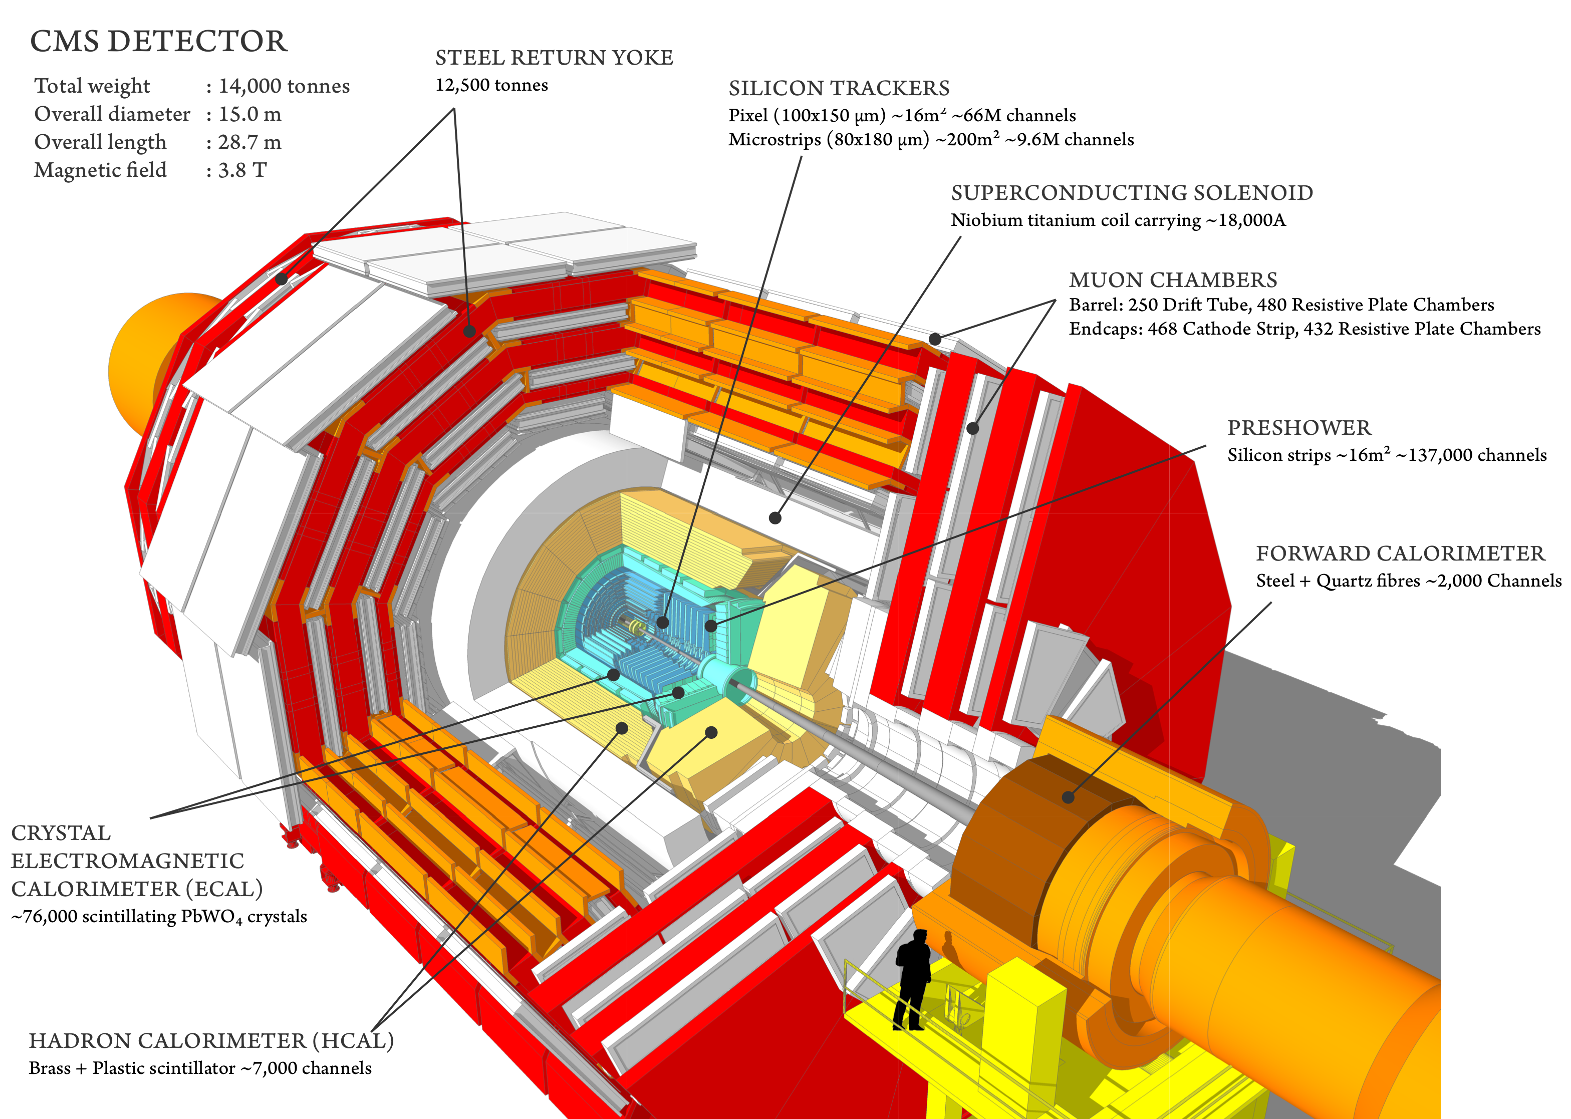
\includegraphics[width=1\textwidth]{figures/detector_system.png}
	\caption{detector system draft}
	\label{fig:detectorsystem}
	\end{figure}
	
	The data are filtered by a two-step triggersystem. The hardware-based system (L1) is triggered when muons, electrons, photons and jets are detected. This reduced the data amount from 40MHz to 100kHz. The software-based system (L2) is triggered by the different energies, type and numbers of particles:
	
\begin{itemize}
  \item lepton has 30/35 GeV
  \item at least 3 jets were detected
  \item at least one of the jets have a b-tag
  \item exactly one photon
\end{itemize}

This reduced the data amount from 100kHz auf 1kHz. The data used during this project was recorded in 2016 at a centre-of mass energy of 13TeV. The signal and background processes were modelled using Monte Carlo generators and passed through a detector simulation (DOUBLE CHECK). 

	\subsection{Proton-Proton-collision and $t\overline{t}\gamma$}
	The protons are accelerated in bunches, each containing 10$^{11}$ particles, through different beam pipes in opposite directions and then collided with each other. The $t\overline{t}\gamma$ events were analysed, meaning top quark pair events with additional photons.
	
	The top quark is the heaviest quark in the known elementary particles and is the only quark so far whose properties can be analysed, since the lifetime is very short and it forms no bound state before it decays. By that the electromagnetic coupling, therefore the number of radiated photons after interaction with other charged particles, can be measured. This is a test of the standard model, since it is a direct measurment of the charge of the top quark and shows possible anomalous structure of its electromagnetic interaction.
	
	During the pp-process a top quark pair is produced. The top quark then decays in a W-boson and a b-quark. The W-boson disintegrates into a charged lepton and a corresponding neutrino or a pair of up-type quark and down-type antiquark. The remaining quarks decomposes into jets. This process can be seen in Figure \ref{fig:PPprocess}.
	
	\begin{figure}[H]
	\centering
	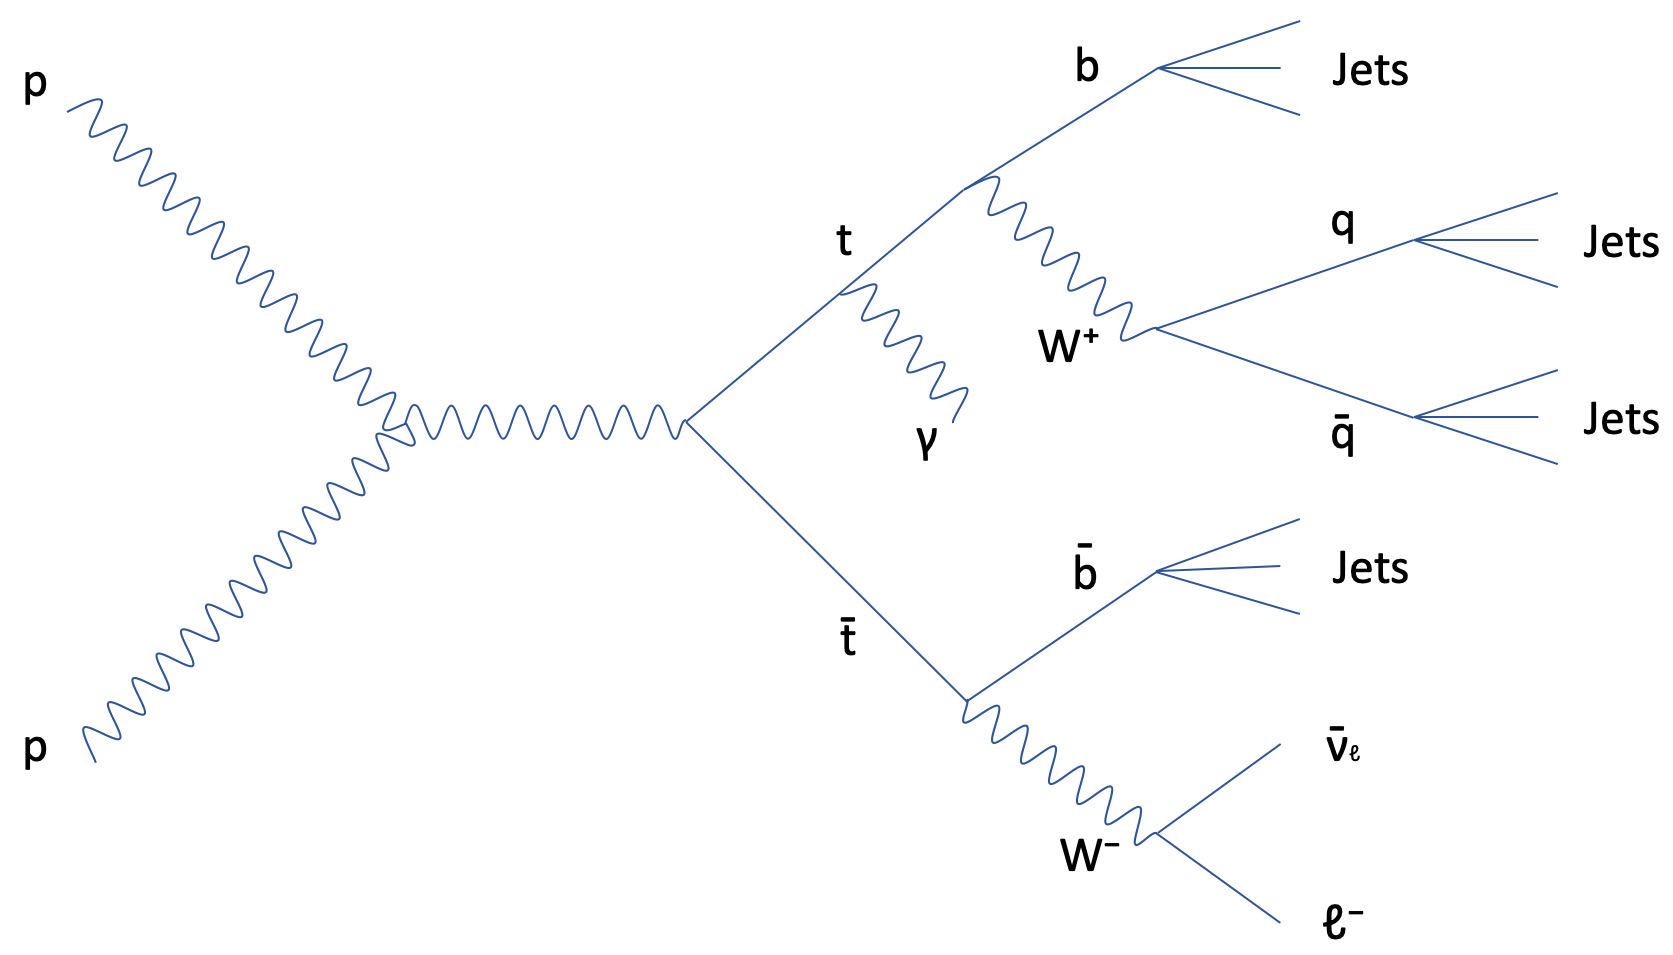
\includegraphics[width=1\textwidth]{figures/PP_process.png}
	\caption{PP process draft}
 	\label{fig:PPprocess}
	\end{figure}
	
\section{Challenge in categorisation}

In Figure \ref{fig:PhotonPT}, the transverse momentum of the photon is visible. The background makes up nearly 50\% of the signal region. These are made up by particles, which were misconstructed or not detected due to the limited detector's acceptence. Other reasons are photons not being radiated from the $t\overline{t}$ process, but rather from an initial charged patron, an intermediate top quark or any charged final state particles or decay products. Further sources could be hadrons misreconstructed as electrons or hadrons and electrons misidentified as photons. 

\begin{figure}[H]
\centering
\begin{minipage}{.5\textwidth}
  \centering
  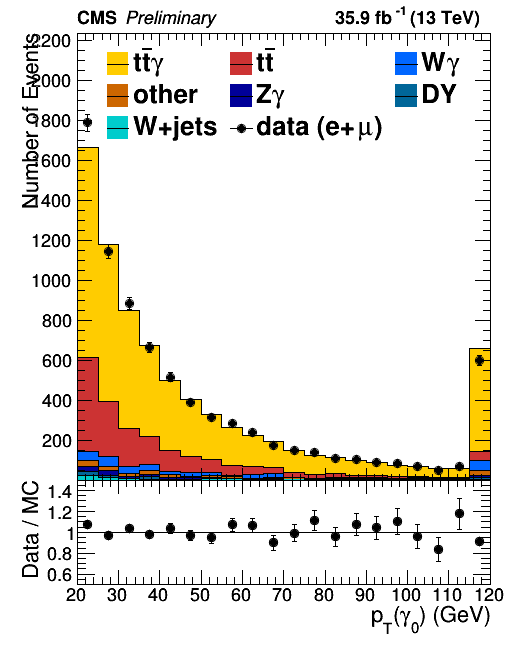
\includegraphics[width=1\linewidth]{figures/PhotonGood0_pt_lin.png}
  \captionof{figure}{Distribution of Pt Photon}
  \label{fig:PhotonPT}
\end{minipage}%
\begin{minipage}{.5\textwidth}
  \centering
  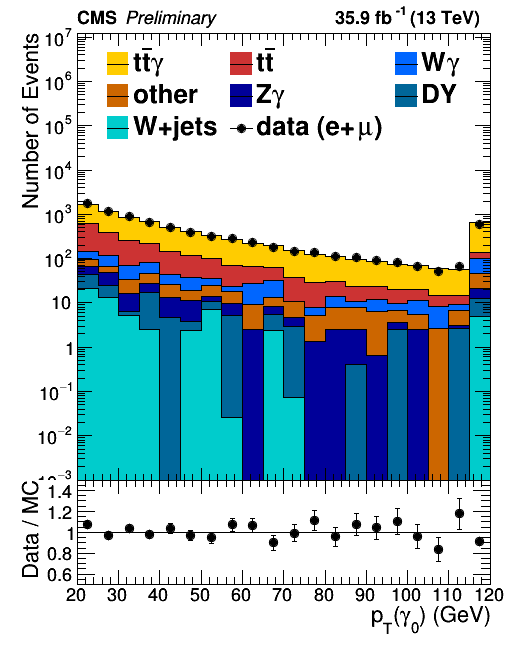
\includegraphics[width=1\linewidth]{figures/PhotonGood0_pt_log.png}
  \captionof{figure}{Distribution of Pt Photon (log)}
  \label{fig:PhotonPTlog}
\end{minipage}
\end{figure}

	\subsection{Current status}
	
	First a neural network was developed to seperate the hadronic-fake photons, which are hadrons misidentified as photons and made up the majority of the background signal. The result was then used as an input for the neural network created to split the $t\overline{t}\gamma$ signal and the background further. What still needs to be further investigated is the possibility of improvement in the discrimination between $t\overline{t}\gamma$ and $t\overline{t}$ events in the signal region through MVAs.

\section{Analysis process}

	\subsection{List of variables}
	
The analysed variables are listed below and they are categorized by the type of particles. 

\begin{itemize}
  \item B-jet: variables of jets containing b-hadrons (b-tag)
	\begin{AutoMultiColItemize}
  		\item Bj0\_eta
  		\item Bj0\_phi
  		\item Bj0\_pt
  		\item Bj1\_eta
  		\item Bj1\_phi
  		\item Bj1\_pt
  		\item nBTagGood
	 \end{AutoMultiColItemize}
  \item Jet: variables of all jets 
  	\begin{AutoMultiColItemize}
  		\item JetGood0\_eta
  		\item JetGood0\_phi
  		\item JetGood0\_pt
  		\item JetGood1\_eta
  		\item JetGood1\_phi
  		\item JetGood1\_pt
  		\item nJet
  		\item nJetGood
  		\item JetGood0\_neEmEF
		\item JetGood0\_chEmEF
		\item JetGood0\_neHEF
		\item JetGood0\_chHEF
 	\end{AutoMultiColItemize}
  \item Lepton: variables of electron, muon
    	\begin{AutoMultiColItemize}
  		\item LeptonTight0\_eta
  		\item LeptonTight0\_phi
  		\item LeptonTight0\_pt
  		\item nElectronTight
  		\item nLeptonTight
  		\item nMuonTight
  		\item LeptonTight0\_pfRelIso03\_all
		\item LeptonTight0\_pfRelIso03\_chg
		\item LeptonTight0\_pfRelIso03\_ne
 	\end{AutoMultiColItemize}
  \item Combination: variables of two particle types 
  	\begin{AutoMultiColItemize}
		\item leptonJetdR
		\item tightLeptonJetdR
		\item ltight0GammadPhi
		\item ltight0GammadR
		\item PhotonLepdR
		\item PhotonJetdR
		\item JetGood0\_btagDeepB
		\item JetGood1\_btagDeepB
	\end{AutoMultiColItemize}
  \item Photon:
  	\begin{AutoMultiColItemize}
  		\item nHighPTPhotons
		\item nPhotonGood
		\item PhotonGood0\_eta
		\item PhotonGood0\_mvaID
		\item PhotonGood0\_phi
		\item PhotonGood0\_pt
		\item PhotonGood0\_sieie
		\item PhotonGood0\_hoe
		\item PhotonGood0\_r9
		\item PhotonGood0\_pfRelIso03\_all
		\item PhotonGood0\_pfRelIso03\_chg
		\item PhotonGood0\_pfRelIso03\_ne
   	\end{AutoMultiColItemize}
  \item Others: 
	\begin{AutoMultiColItemize}
  		\item MET\_phi
  		\item MET\_pt
		\item ht
		\item m3
		\item mT
 	\end{AutoMultiColItemize}
\end{itemize}

The pre- or suffix of the name reveal, what information is saved. The description of variables, which don't follow this logic, are listed at the end. 

Prefix and suffix:
\begin{itemize}
	  \item \_eta: pseudorapidity ($\eta = -ln(tan(\frac{\vartheta}{2}))$; wheras $\vartheta$ is the polar angle)
	  \item \_phi: azithmuthal opening angle, around z-axis ($\Delta\phi$)
	  \item \_pt: transverse momentum of variable
	  \item dR: distance between two objects ($\Delta$R)
	  \item n: number of particles
\end{itemize}

Other:
\begin{itemize}
  \item ht
  \item m3
  \item mT
  \item PhotonGood0: number of photons
  \item MVA\_ID: currently used as a parameter to differentiate between good and bad photon (??)
  \item MET: Missing transverse momentum
\end{itemize}

	\subsection{Analysis of variables}
	
The variables were analysed by comparing the distribution of events with an uniform scaling. A uniform scaling was needed to have a better view of relative differences between signal and background. If the variable shows a different behaviour for each type of signal, this could be an indication of discriminatory power. 

Figure \ref{fig:Bj0eta} to \ref{fig:LeptonTight0eta} show some examples of variables, where the distributions are almost identical and were therefore not further analysed. A full list of these variables are listed in the Annex, chapter \ref{sec:annex-identical}. 

\begin{figure}[H]
\centering
\begin{minipage}{.5\textwidth}
  \centering
  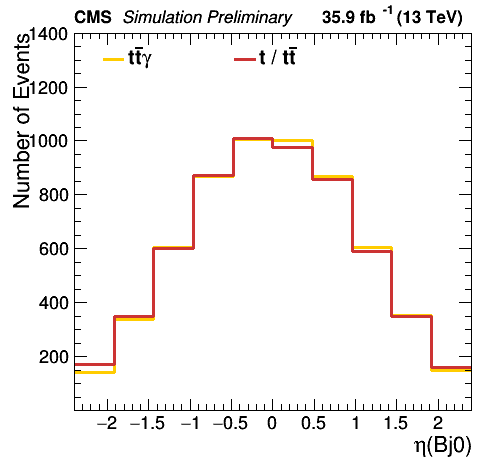
\includegraphics[width=0.75\linewidth]{figures/Notused/Bj0_eta.png}
  \captionof{figure}{Bj0\_eta}
  \label{fig:Bj0eta}
\end{minipage}%
\begin{minipage}{.5\textwidth}
  \centering
  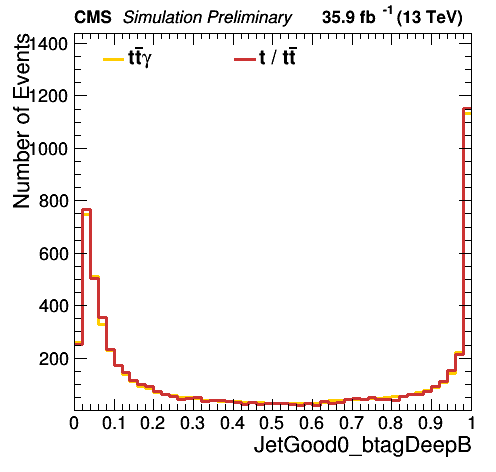
\includegraphics[width=0.75\linewidth]{figures/Notused/JetGood0_btagDeepB.png}
  \captionof{figure}{JetGood0\_btagDeepB}
  \label{fig:JetGood0btagDeepB}
\end{minipage}
\end{figure}

\begin{figure}[H]
\centering
\begin{minipage}{.5\textwidth}
  \centering
  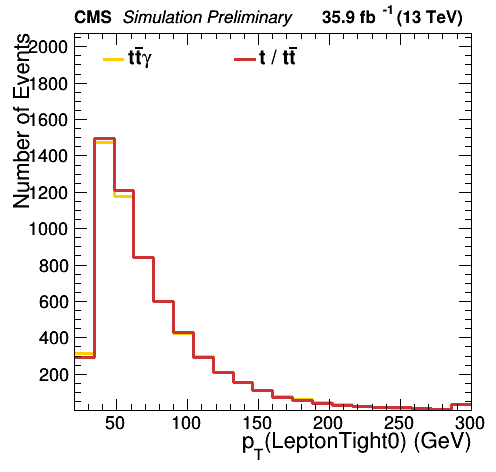
\includegraphics[width=0.75\linewidth]{figures/Notused/LeptonTight0_pt.png}
  \captionof{figure}{LeptonTight0\_pt}
  \label{fig:LeptonTight0pt}
\end{minipage}%
\begin{minipage}{.5\textwidth}
  \centering
  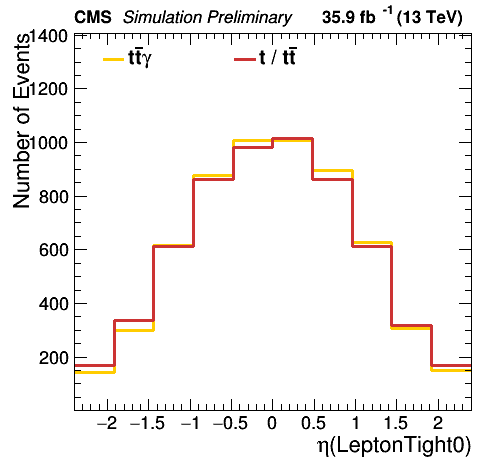
\includegraphics[width=0.75\linewidth]{figures/Notused/LeptonTight0_eta.png}
  \captionof{figure}{LeptonTight0\_eta}
  \label{fig:LeptonTight0eta}
\end{minipage}
\end{figure}

In Figure \ref{fig:nBTagGood} to \ref{fig:ht} there are some differences visible in the signal region. These were candidates for the first set of selected variables. 

	\begin{figure}[H]
	\centering
	\begin{minipage}{.5\textwidth}
	  \centering
	  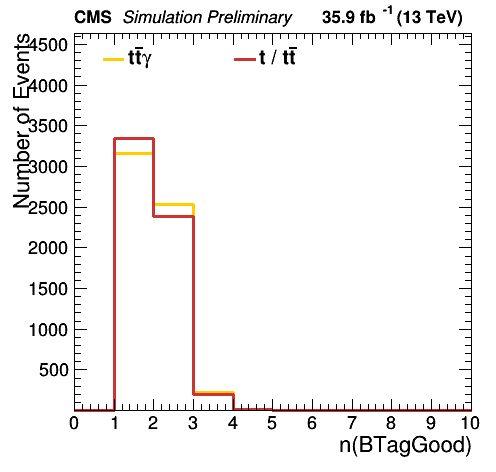
\includegraphics[width=0.75\linewidth]{figures/Select1/nBTagGood.png}
	  \captionof{figure}{nBTagGood}
	  \label{fig:nBTagGood}
	\end{minipage}%
	\begin{minipage}{.5\textwidth}
	  \centering
	  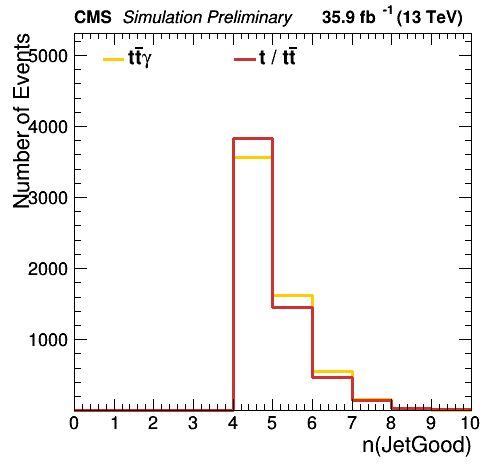
\includegraphics[width=0.75\linewidth]{figures/Select1/nJetGood.png}
	  \captionof{figure}{nJetGood}
	  \label{fig:nJetGood}
	\end{minipage}
	\end{figure}
	
	\begin{figure}[H]
	\centering
	\begin{minipage}{.5\textwidth}
	  \centering
	  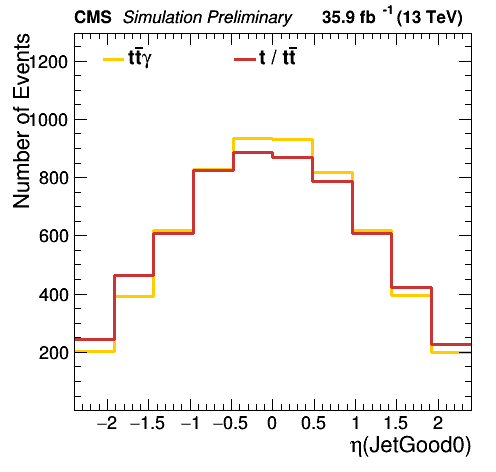
\includegraphics[width=0.75\linewidth]{figures/Select1/JetGood0_eta.png}
	  \captionof{figure}{JetGood0\_eta}
	  \label{fig:JetGood0eta}
	\end{minipage}%
	\begin{minipage}{.5\textwidth}
	  \centering
	  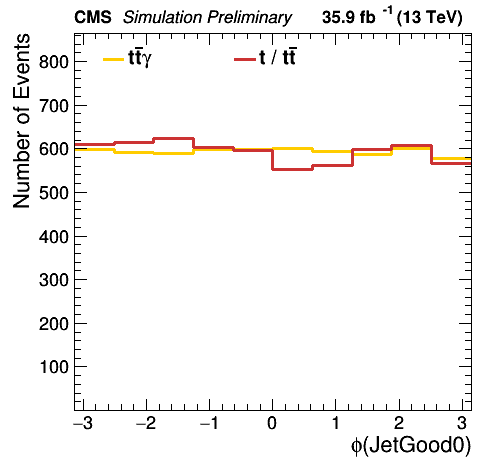
\includegraphics[width=0.75\linewidth]{figures/Select1/JetGood0_phi.png}
	  \captionof{figure}{JetGood0\_phi}
	  \label{fig:JetGood0phi}
	\end{minipage}
	\end{figure}
	
	\begin{figure}[H]
	\centering
	\begin{minipage}{.5\textwidth}
	  \centering
	  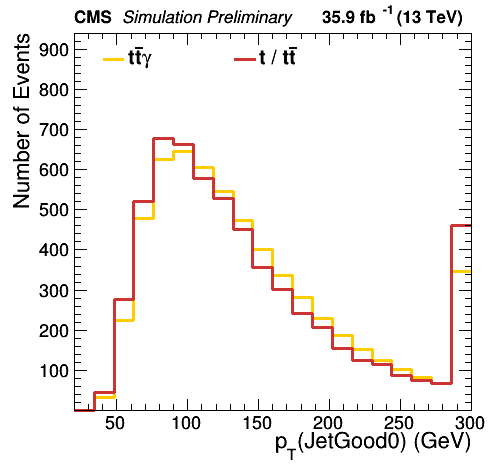
\includegraphics[width=0.75\linewidth]{figures/Select1/JetGood0_pt.png}
	  \captionof{figure}{JetGood0\_pt}
	  \label{fig:JetGood0pt}
	\end{minipage}%
	\begin{minipage}{.5\textwidth}
	  \centering
	  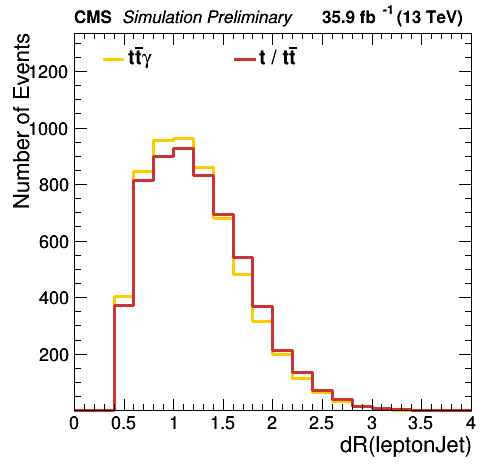
\includegraphics[width=0.75\linewidth]{figures/Select1/leptonJetdR.png}
	  \captionof{figure}{leptonJetdR}
	  \label{fig:leptonJetdR}
	\end{minipage}
	\end{figure}
	
	\begin{figure}[H]
	\centering
	\begin{minipage}{.5\textwidth}
	  \centering
	  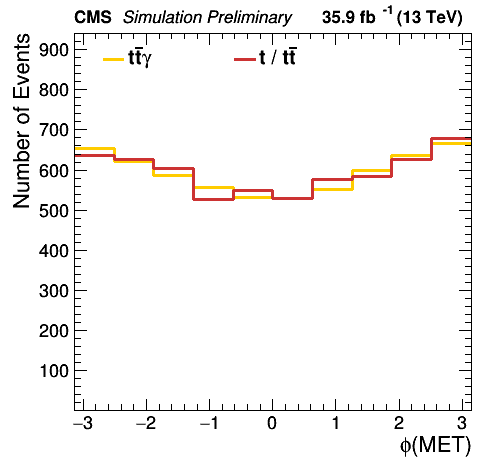
\includegraphics[width=0.75\linewidth]{figures/Select1/MET_phi.png}
	  \captionof{figure}{MET\_phi}
	  \label{fig:METphi}
	\end{minipage}%
	\begin{minipage}{.5\textwidth}
	  \centering
	  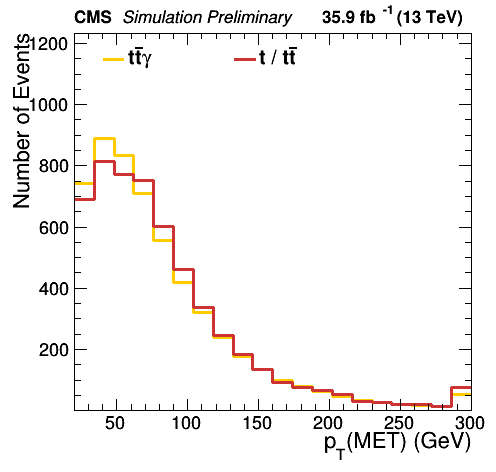
\includegraphics[width=0.75\linewidth]{figures/Select1/MET_pt.png}
	  \captionof{figure}{MET\_pt}
	  \label{fig:METpt}
	\end{minipage}
	\end{figure}
	
	\begin{figure}[H]
	\centering
	\begin{minipage}{.5\textwidth}
	  \centering
	  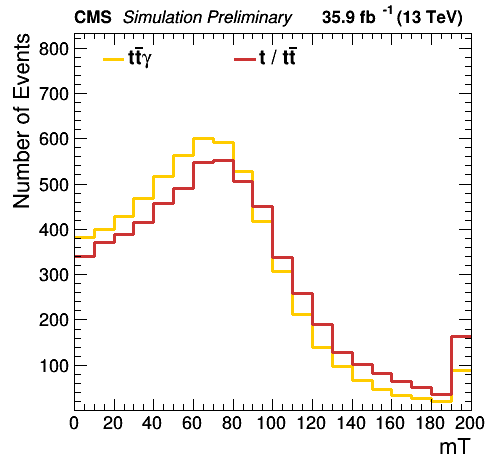
\includegraphics[width=0.75\linewidth]{figures/Select1/mT.png}
	  \captionof{figure}{mT}
	  \label{fig:mT}
	\end{minipage}%
	\begin{minipage}{.5\textwidth}
	  \centering
	  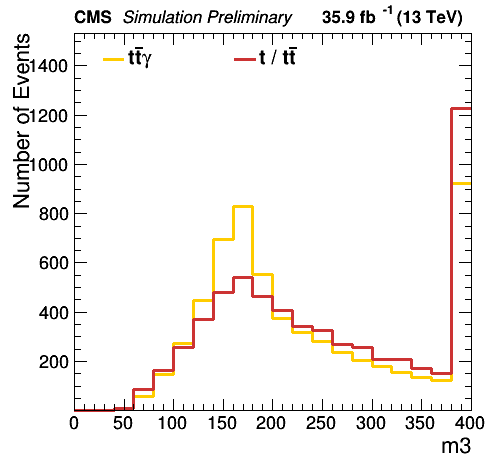
\includegraphics[width=0.75\linewidth]{figures/Select1/m3.png}
	  \captionof{figure}{m3}
	  \label{fig:m3}
	\end{minipage}
	\end{figure}

	\begin{figure}[H]
	\centering
	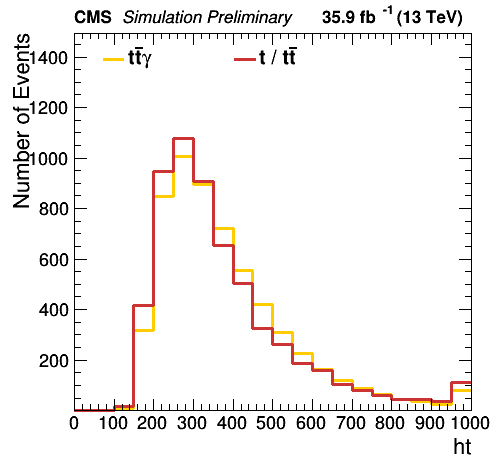
\includegraphics[width=0.38\textwidth]{figures/Select1/ht.png}
	\caption{ht}
 	\label{fig:ht}
	\end{figure}
	
The variable MVA\_ID, seen in figure \ref{fig:PhotonGood0mvaID}, shows quite a good distinction and is therefore used in the second selection.

	\begin{figure}[H]
	\centering
	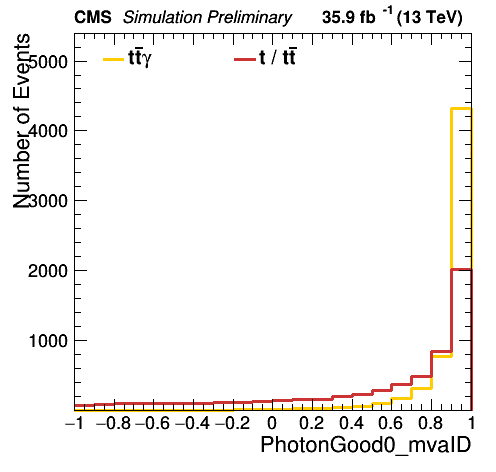
\includegraphics[width=0.38\textwidth]{figures/Select2/PhotonGood0_mvaID.png}
	\caption{PhotonGood0\_mvaID}
 	\label{fig:PhotonGood0mvaID}
	\end{figure}
	
Figure \ref{fig:PhotonGood0pt} to \ref{fig:PhotonGood0pfRelIso03all} show the photon variables. These show the most promising behaviour for discrimination between $t\overline{t}\gamma$ and $t\overline{t}$ events and were put into the third selection category.

	\begin{figure}[H]
	\centering
	\begin{minipage}{.5\textwidth}
	  \centering
	  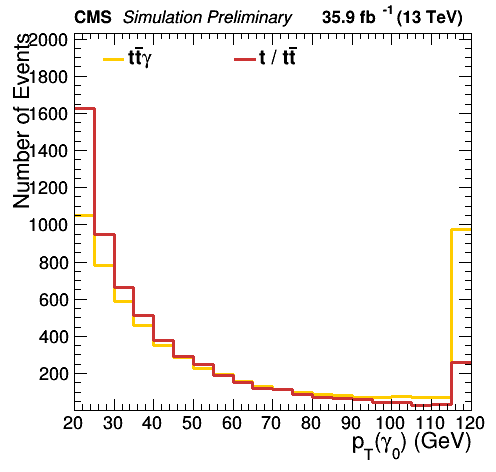
\includegraphics[width=0.75\linewidth]{figures/Select3/PhotonGood0_pt.png}
	  \captionof{figure}{PhotonGood0\_pt}
	  \label{fig:PhotonGood0pt}
	\end{minipage}%
	\begin{minipage}{.5\textwidth}
	  \centering
	  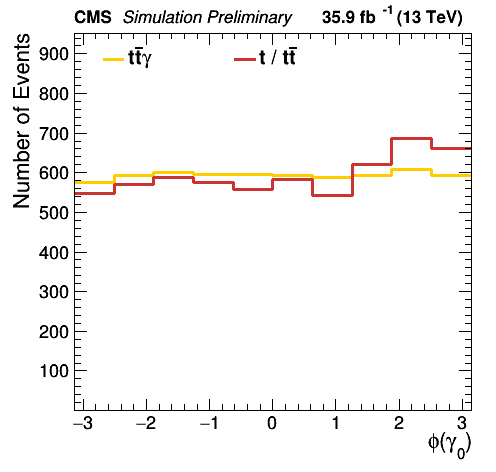
\includegraphics[width=0.75\linewidth]{figures/Select3/PhotonGood0_phi.png}
	  \captionof{figure}{PhotonGood0\_phi}
	  \label{fig:PhotonGood0phi}
	\end{minipage}
	\end{figure}
	
	\begin{figure}[H]
	\centering
	\begin{minipage}{.5\textwidth}
	  \centering
	  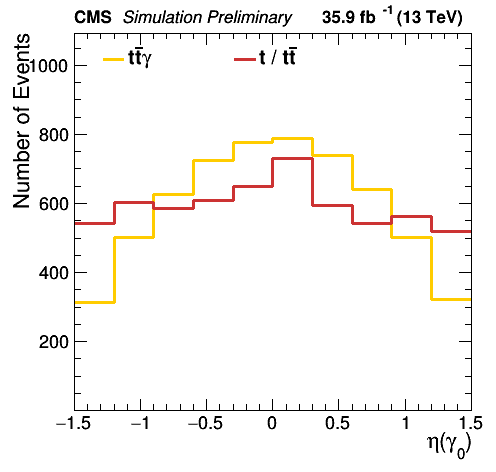
\includegraphics[width=0.75\linewidth]{figures/Select3/PhotonGood0_eta.png}
	  \captionof{figure}{PhotonGood0\_eta}
	  \label{fig:PhotonGood0eta}
	\end{minipage}%
	\begin{minipage}{.5\textwidth}
	  \centering
	  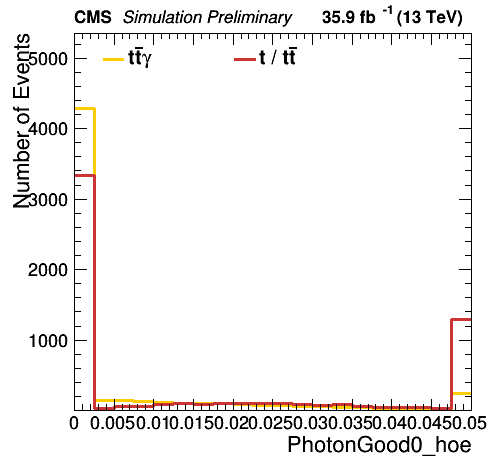
\includegraphics[width=0.75\linewidth]{figures/Select3/PhotonGood0_hoe.png}
	  \captionof{figure}{PhotonGood0\_hoe}
	  \label{fig:PhotonGood0hoe}
	\end{minipage}
	\end{figure}
	
	\begin{figure}[H]
	\centering
	\begin{minipage}{.5\textwidth}
	  \centering
	  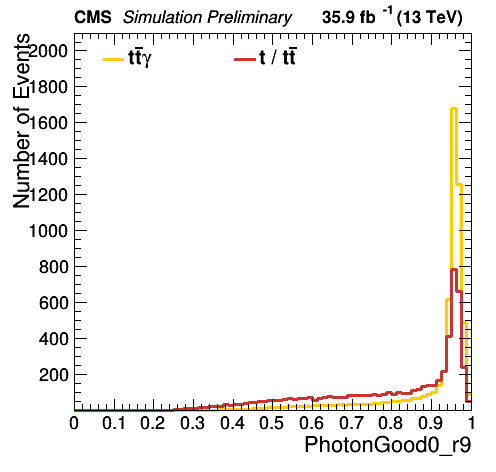
\includegraphics[width=0.75\linewidth]{figures/Select3/PhotonGood0_r9.png}
	  \captionof{figure}{PhotonGood0\_r9}
	  \label{fig:PhotonGood0r9}
	\end{minipage}%
	\begin{minipage}{.5\textwidth}
	  \centering
	  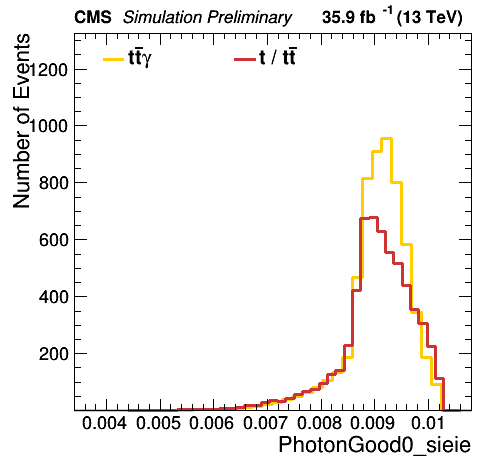
\includegraphics[width=0.75\linewidth]{figures/Select3/PhotonGood0_sieie.png}
	  \captionof{figure}{PhotonGood0\_sieie}
	  \label{fig:PhotonGood0sieie}
	\end{minipage}
	\end{figure}
	
	\begin{figure}[H]
	\centering
	\begin{minipage}{.5\textwidth}
	  \centering
	  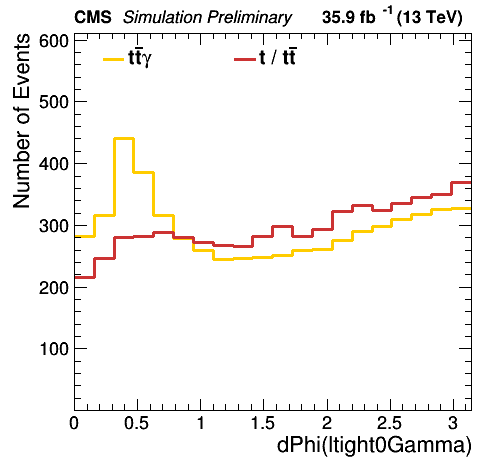
\includegraphics[width=0.75\linewidth]{figures/Select3/ltight0GammadPhi.png}
	  \captionof{figure}{ltight0GammadPhi}
	  \label{fig:ltight0GammadPhi}
	\end{minipage}%
	\begin{minipage}{.5\textwidth}
	  \centering
	  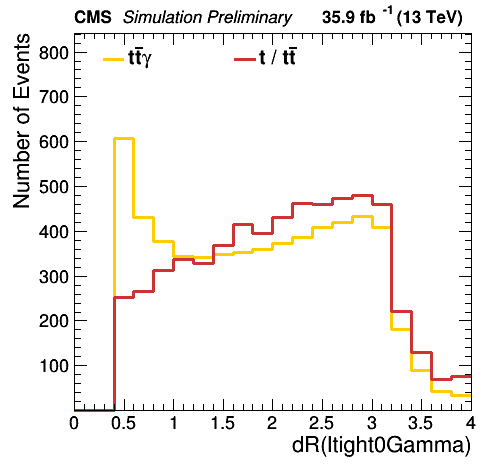
\includegraphics[width=0.75\linewidth]{figures/Select3/ltight0GammadR.png}
	  \captionof{figure}{ltight0GammadR}
	  \label{fig:ltight0GammadR}
	\end{minipage}
	\end{figure}
	
	\begin{figure}[H]
	\centering
	\begin{minipage}{.5\textwidth}
	  \centering
	  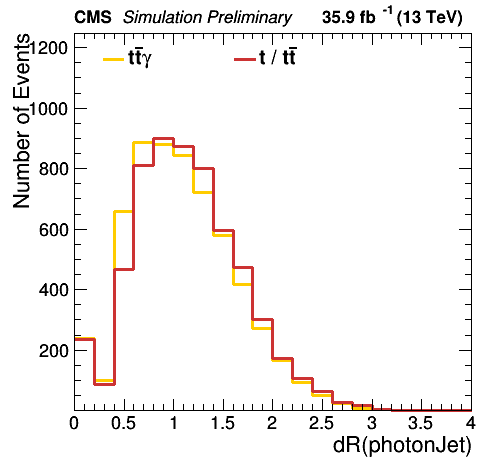
\includegraphics[width=0.75\linewidth]{figures/Select3/photonJetdR.png}
	  \captionof{figure}{photonJetdR}
	  \label{fig:photonJetdR}
	\end{minipage}%
	\begin{minipage}{.5\textwidth}
	  \centering
	  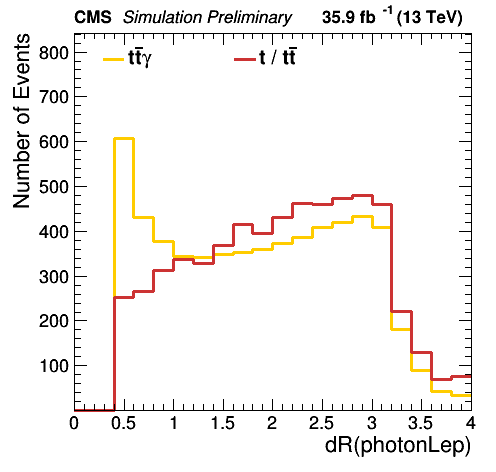
\includegraphics[width=0.75\linewidth]{figures/Select3/photonLepdR.png}
	  \captionof{figure}{photonLepdR}
	  \label{fig:photonLepdR}
	\end{minipage}
	\end{figure}

	\begin{figure}[H]
	\centering
	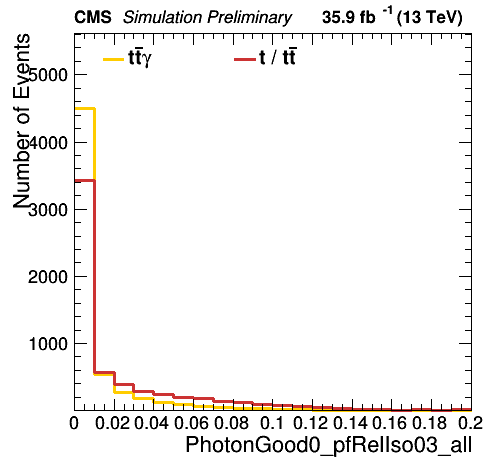
\includegraphics[width=0.38\textwidth]{figures/Select3/PhotonGood0_pfRelIso03_all.png}
	\caption{PhotonGood0\_pfRelIso03\_all}
 	\label{fig:PhotonGood0pfRelIso03all}
	\end{figure}

Variables, which were excluded because another related variable was used instead, are listed in the Annex, chapter \ref{sec:annex-excluded}. 

\section{MVA}

Trying to split signal and background through a variable with a cut-off value faces the problem, that this criteria doesn't apply for every event. If it works for one event, it doesn't mean that it works for the next one. Therefore mutliple variables need to be used to distinguish between those two categories, so called multivariate analysis (MVA). As already mentioned in chapter \ref{sec:approach}, the chosen MVA-types are boosted decision trees (BDT) and multilayer perceptron (MLP).

	\subsection{BDT - Boosted Decision Trees}
	The decision tree starts with the root node containing the whole sample For a binary tree, the node is then split into two branches using a variable and a corresponding cut-off value. The cut-off value should be a value, which seperates the signal from the background the best. This process will be repeated for each branch for all relevant variables, including already used variables, until an end criteria is met. The final branch is called a leaf and this will be assigned to one of the two categories. End criterias could be a minimum size of a leaf, perfect separation, insignificant improvement after split or maximal tree depth. Boosted decision trees are built out of additional trees, so called weak classifieres. They include variables with a low discriminatory power and will be used to improve the main decision tree to a more stable model with a lower error rate. 

	\begin{figure}[H]
	\centering
	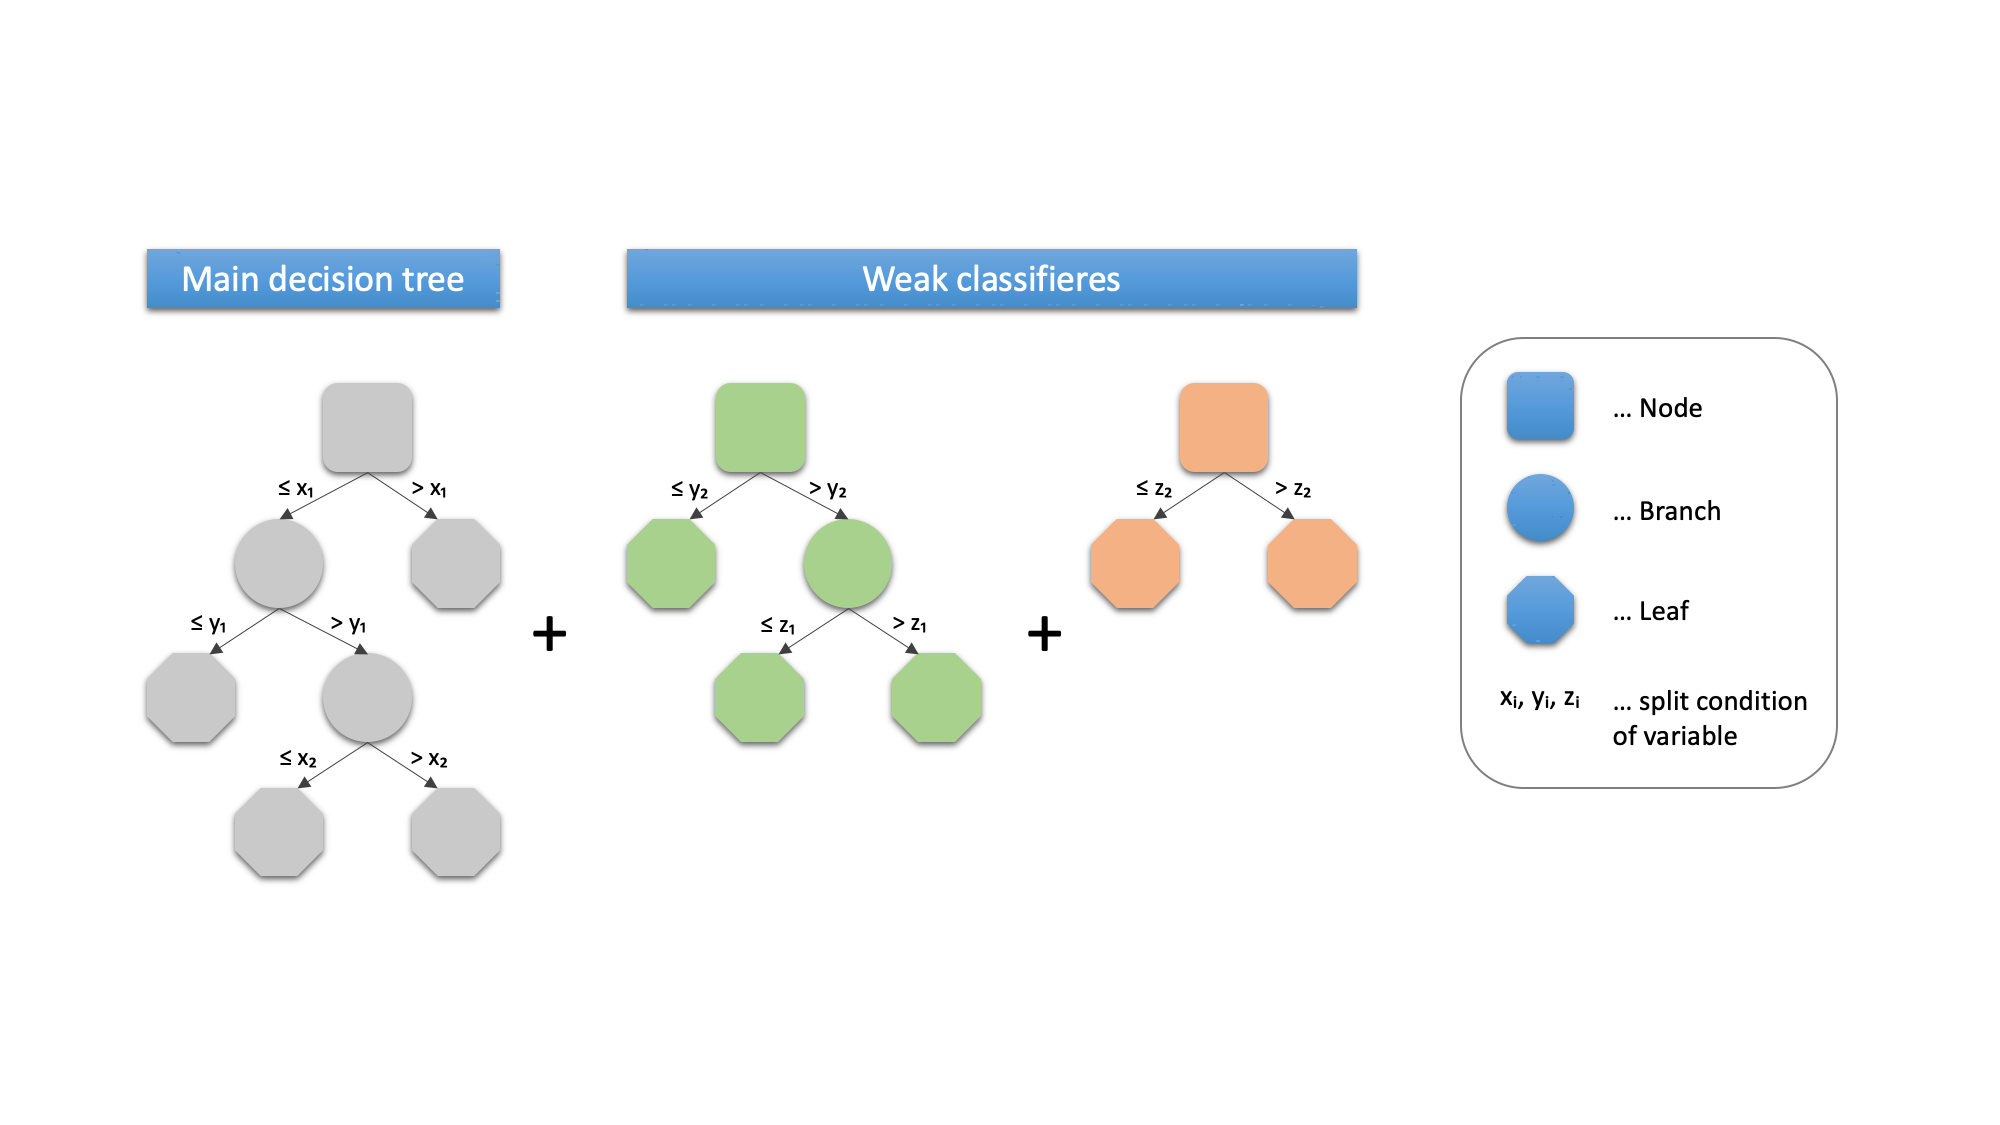
\includegraphics[width=1\textwidth]{figures/BDT.png}
	\caption{PP process draft}
	\end{figure}
	
	\subsection{MLP - Multilayer Perceptron}
	
	The model is built out of multiple perceptrons, which are arranged in layers shown in Figure \ref{fig:MLP}. The value of one perceptron is the sum of all weighted inputs. This value is then transformed through an activation function and a treshhold. The activation funtion is a linear function for the input- and outputlayer, while for the hiddenlayers it is usually the log-sigmoid transfer function, seen in figure \ref{fig:log-sigmoid function}. All layers have a treshhold, except the inputlayer. 
	
	\begin{figure}[H]
	\centering
	\begin{minipage}{.5\textwidth}
	  \centering
	  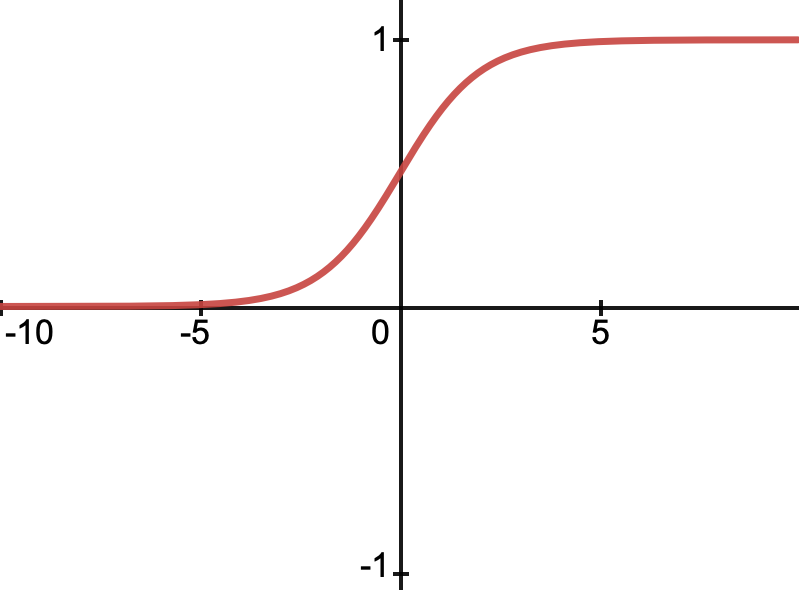
\includegraphics[width=0.75\linewidth]{figures/log-sigmoid.png}
	  %\captionof{figure}{log-sigmoid function}
	  %\label{fig:log-sigmoid function}
	\end{minipage}%
	\begin{minipage}{.5\textwidth}
	  \centering
		\begin{equation*}
			f(x) = \frac{1}{1 +e^{-x}}
		\end{equation*}
	  %\captionof{equation}{photonLepdR}
	\end{minipage}
	\captionof{figure}{log-sigmoid function}
	\label{fig:log-sigmoid function}
	\end{figure}
	
	In the MLP, every perceptron of a layer is connected to every perceptron of the previous and next layer. Each connection has an assigned weight, so called weight coefficient. All coefficients of one layer can be written as a weight matrix. The first and layer are called input- and outputlayer respectively, while the intermediate layers are the hiddenlayers. A MLP has a minimum of one hiddenlayer, therefore contains at least three layers.
	
	If the signal is only transmitted in one direction, therefore the MLP doesn't have loops, it is described as feed forward. The learning process of the model is called backpropagation algorithm. It learns by minimizing the error between network output and expexted output. Initially all weights are assigned random values, then every event will go through the network and the weights are adapted. Either all events will be put through the network first and then the values are adapted or are adjusted after each event, but for the latter the order of the events might be important. After one epoch the end criteria will be tested. If it fails, the whole learning process will be carried out again. If it is met, the algorithm is finished.
	
\begin{figure}[H]
	\begin{center}
	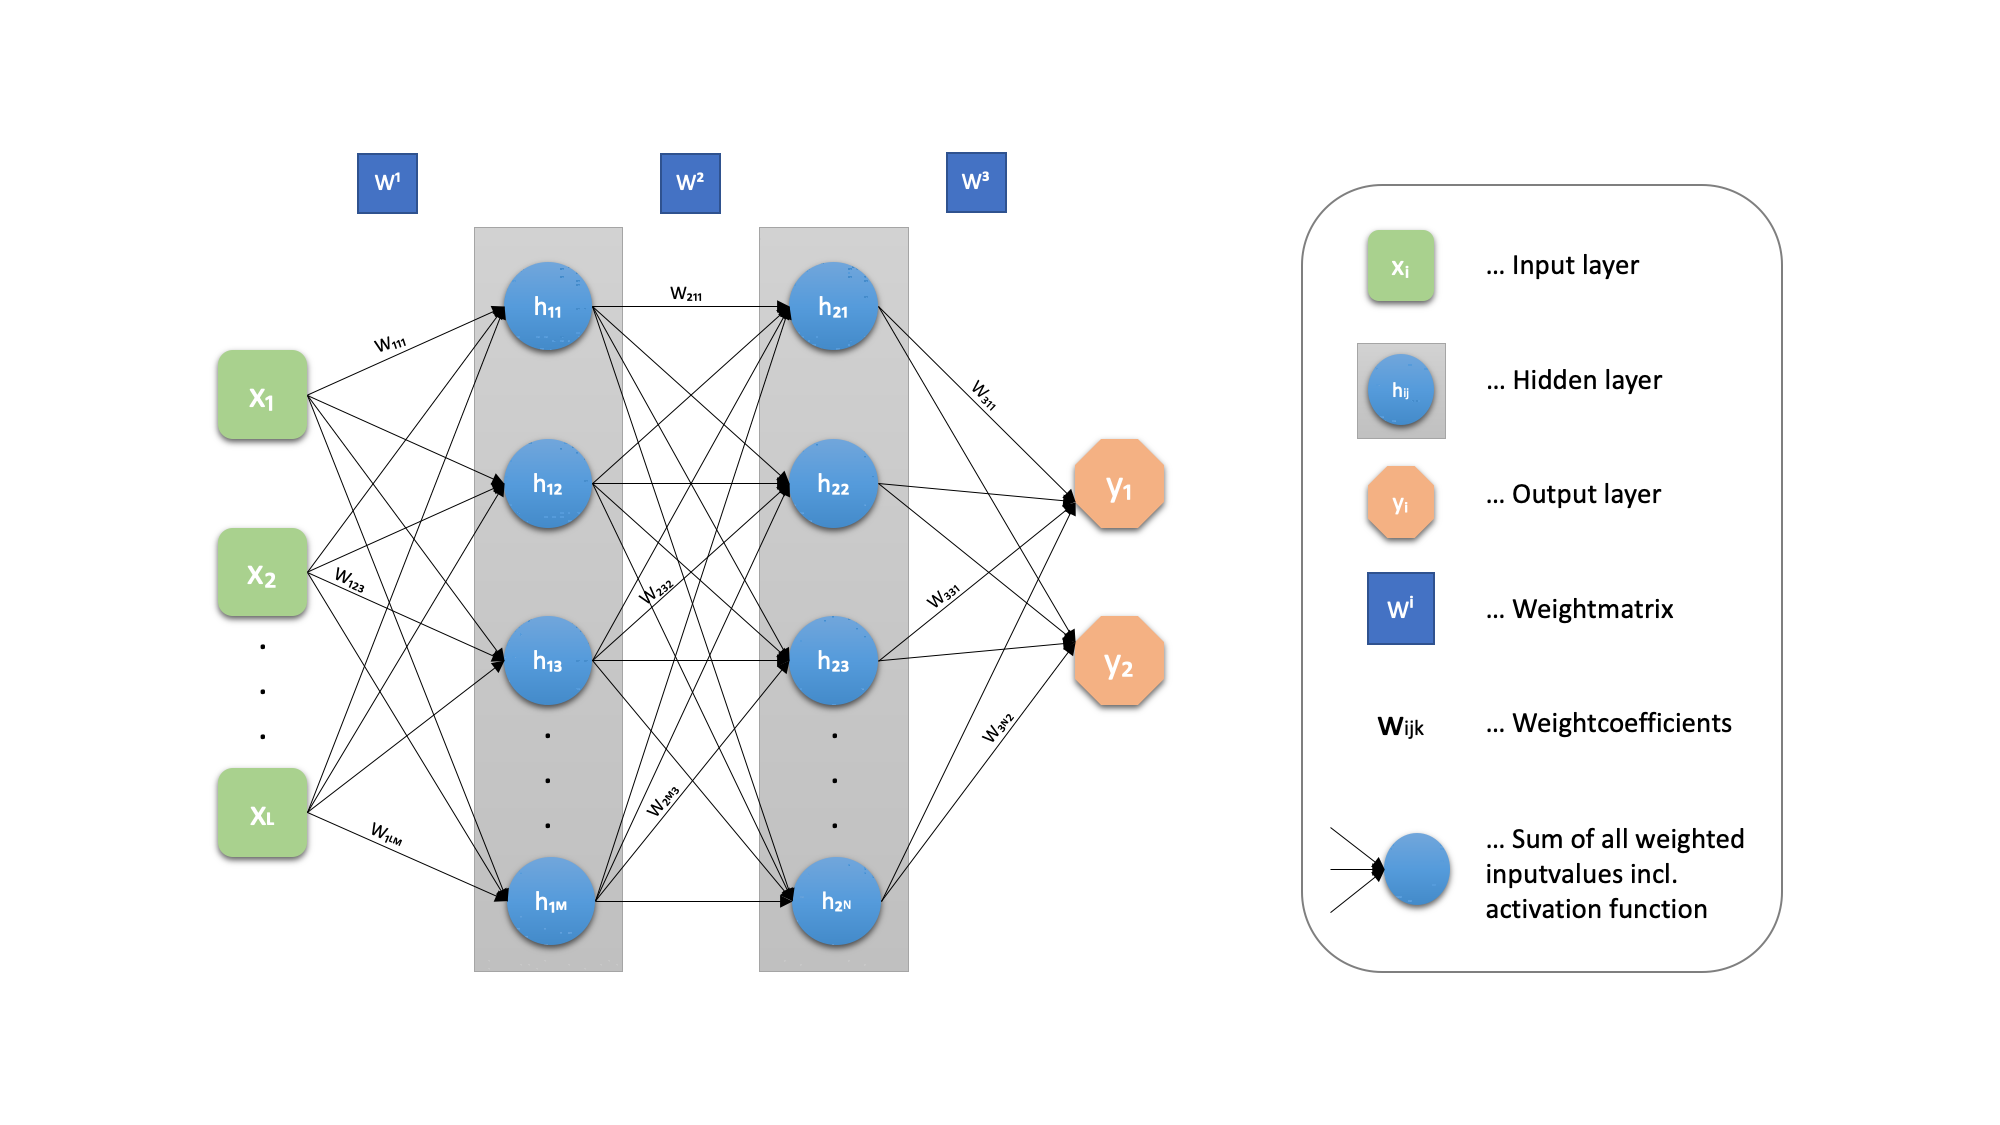
\includegraphics[width=1\textwidth]{figures/MLP.png}
	\caption{MLP draft}
	\label{fig:MLP}
	\end{center}
\end{figure}

	\subsection{Training of MVA}
	
	The following table shows some of the default values used for the models.
	
		\begin{itemize}
  			\item BDT
  					\begin{itemize}
  					\item Minimum node size
  					\item Separation type
  					\end{itemize}
  		  	\item MLP
  					\begin{itemize}
  					\item Number of cycles
  					\item Learning Rate
  					\item Decayrate
  					\item Neurontype
  					\item Estimatortype
  					\item Neuroninputtype
  					\item Trainingmethod
  					\end{itemize}		
		\end{itemize}
		
	A full list of all parameters, configuration options as well as their default values are given in the annex, chapter xx.
	
	These parameters were adapted to improve the result:
		\begin{itemize}
  			\item BDT
  					\begin{itemize}
  					\item Maximum depth
  					\item Number of trees
  					\item Number of Cuts
  					\end{itemize}
  		  	\item MLP
  					\begin{itemize}
  					\item Number of layers
  					\end{itemize}		
		\end{itemize}
		
	The default values was used as basis. Additionally, the MVAs were trained with a lower and a higher configuration:
	
	\begin{table}[H]
	\begin{tabular}{|l|l|l|l|l|}
	\hline
	              & \multicolumn{3}{c|}{BDT}                         & \multicolumn{1}{c|}{MLP} \\ \hline
	Configuration & maximum depth & number of trees & number of cuts & number of layers         \\ \hline
	1             & 1             & 400             & 10             & 5                        \\ \hline
	2             & 3             & 800             & 25             & 7                        \\ \hline
	3             & 5             & 1000            & 50             & 10                       \\ \hline
	\end{tabular}
	\end{table}

The distribution and ROC-curves for the BDT- and MLP-models are shown for each selection and configuration in the following chapter. To avoid overfitting, each MVA is trained on one part of the sample (training sample) and tested on the rest (testing sample). If the results differ significantly, then this would be a sign of overfitting - the model only differentiates correctly on this specific sample. The results of the train- and test-sample can be seen in the distribution plots.

The ROC-curves show the background rejection versus signal efficiency. While discriminating between signal and background, the signal efficiency is the proportion of the correctly categorized signal events ($t\overline{t}\gamma$) and the background rejection is therefore the correctly assigned fraction of background events ($t\overline{t}$). There are two types of errors during the distinction process:
		\begin{itemize}
  			\item a signal event is categorized as background, which is called false negative
  			\item a background event is assigned to the signal category, calles false positive  			
  		\end{itemize}			
  		
Examples for different types of ROC-curves are displayed in figure \ref{fig:ROC_ex}. The green curve indicate a good discriminatory power. The orange curve show that the model assigns the events the wrong way around. If the ROC-curve follows closely the identity line, then the model doesn't have discriminatory power.

	\begin{figure}[H]
	\centering
	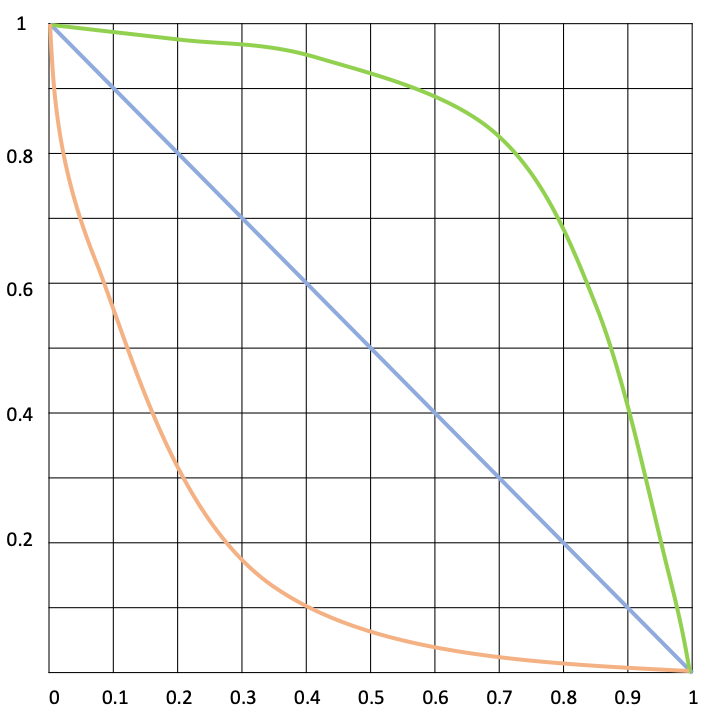
\includegraphics[width=0.5\textwidth]{figures/ROC_curve.png}
	\caption{ROC-curve examples}
	 \label{fig:ROC_ex}	
	\end{figure}
	
	\subsection{Results}
	
	The first selection category were put into the models and are seen in figure \ref{fig:ROC_s1_config1} - \ref{fig:ROC_s1_config3}. A slight improvement in the distinction between $t\overline{t}\gamma$- and $t\overline{t}$-events is visible. 
	
		In the second selection category the variable PhotonGood0mvaID was added (figure \ref{fig:ROC_s2_config1} - \ref{fig:ROC_s2_config3}). The result improved significantly.
		
		Now adding the photon variables for the third selection show a higher success in the distinguishing process. They can be seen in figure \ref{fig:ROC_s3_config1} - \ref{fig:ROC_s3_config3}. 
		
		Between the three configuration combinations there is no significant difference. For all selection categories, the MLP model perfomed better than the BDT model. The third set of variables show the best result.
				
	\begin{figure}[H]
	\centering
	\begin{minipage}{.5\textwidth}
	  \centering
	  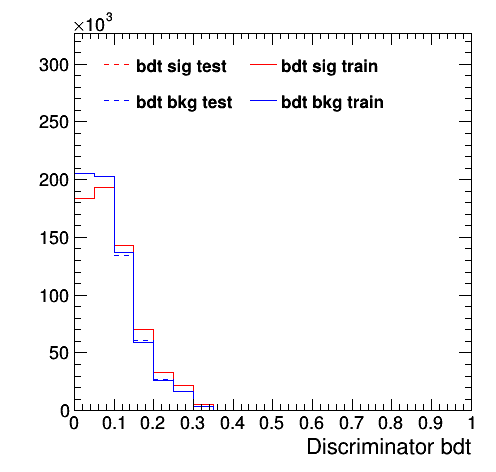
\includegraphics[width=0.75\linewidth]{figures/MVA/select1/config1/discriminator_bdt.png}
	  %\captionof{figure}{BDT distribution for selection 1 variables with configuration 1}
	  \label{fig:distr_s1_config1_bdt}
	\end{minipage}%
	\begin{minipage}{.5\textwidth}
	  \centering
	  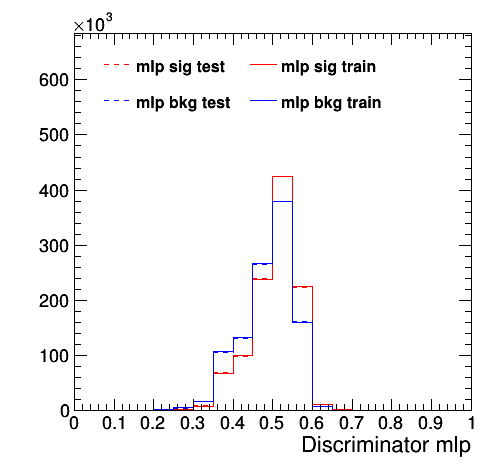
\includegraphics[width=0.75\linewidth]{figures/MVA/select1/config1/discriminator_mlp.png}
	  %\captionof{figure}{MLP distribution for selection 1 variables with configuration 1}
	  \label{fig:distr_s1_config1_mlp}
	\end{minipage}
	\centering
	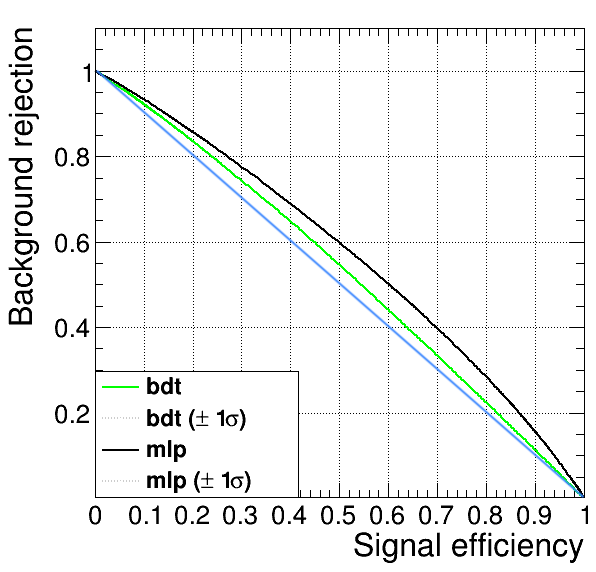
\includegraphics[width=0.5\textwidth]{figures/MVA/select1/config1/FOM_selection1_nL5_nT400_mD1_nC10.png}
	\caption{BDT-, MLP-distribution and ROC curve for variables from selection 1 with configuration 1}
	 \label{fig:ROC_s1_config1}
	\end{figure}
	
	\begin{figure}[H]
	\centering
	\begin{minipage}{.5\textwidth}
	  \centering
	  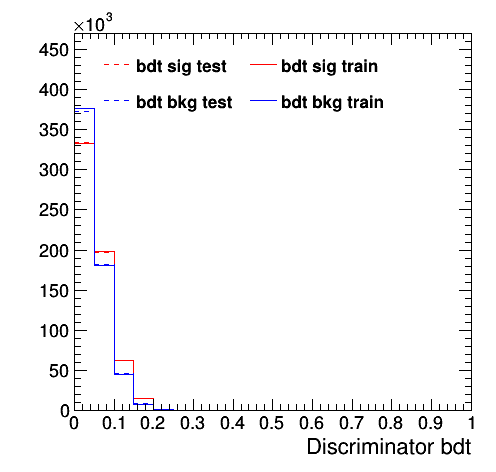
\includegraphics[width=0.75\linewidth]{figures/MVA/select1/config2/discriminator_bdt.png}
	  %\captionof{figure}{BDT distribution for selection 1 variables with configuration 2}
	  \label{fig:distr_s1_config2_bdt}
	\end{minipage}%
	\begin{minipage}{.5\textwidth}
	  \centering
	  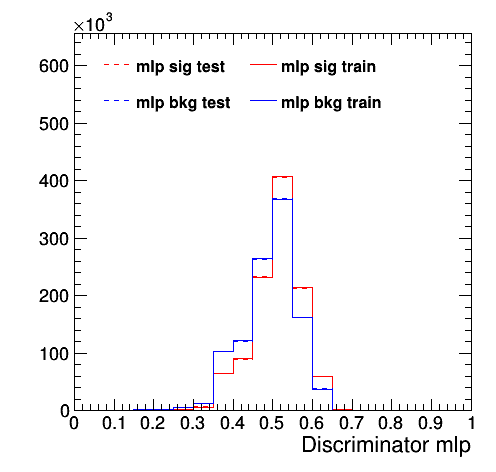
\includegraphics[width=0.75\linewidth]{figures/MVA/select1/config2/discriminator_mlp.png}
	  %\captionof{figure}{MLP distribution for selection 1 variables with configuration 2}
	  \label{fig:distr_s1_config2_mlp}
	\end{minipage}
	\centering
	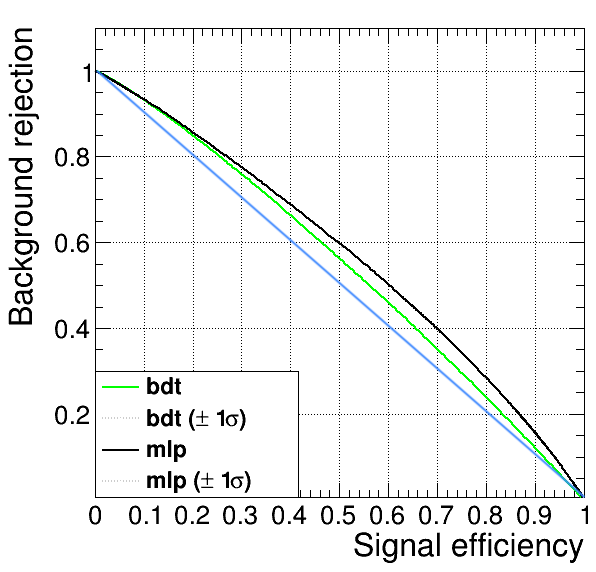
\includegraphics[width=0.5\textwidth]{figures/MVA/select1/config2/FOM_selection1_nL7_nT800_mD3_nC20.png}
	\caption{BDT-, MLP-distribution and ROC curve for variables from selection 1 with configuration 2}
	 \label{fig:ROC_s1_config2}
	\end{figure}
	
	\begin{figure}[H]
	\centering
	\begin{minipage}{.5\textwidth}
	  \centering
	  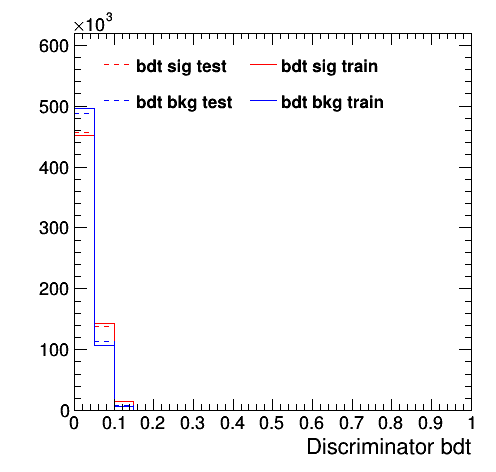
\includegraphics[width=0.75\linewidth]{figures/MVA/select1/config3/discriminator_bdt.png}
	  %\captionof{figure}{BDT distribution for selection 1 variables with configuration 3}
	  \label{fig:distr_s1_config3_bdt}
	\end{minipage}%
	\begin{minipage}{.5\textwidth}
	  \centering
	  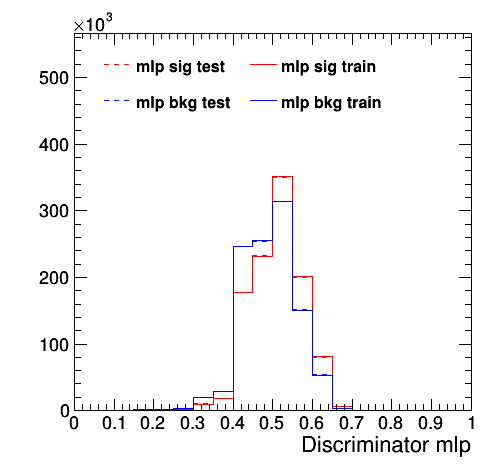
\includegraphics[width=0.75\linewidth]{figures/MVA/select1/config3/discriminator_mlp.png}
	  %captionof{figure}{MLP distribution for selection 1 variables with configuration 3}
	  \label{fig:distr_s1_config3_mlp}
	\end{minipage}
	\centering
	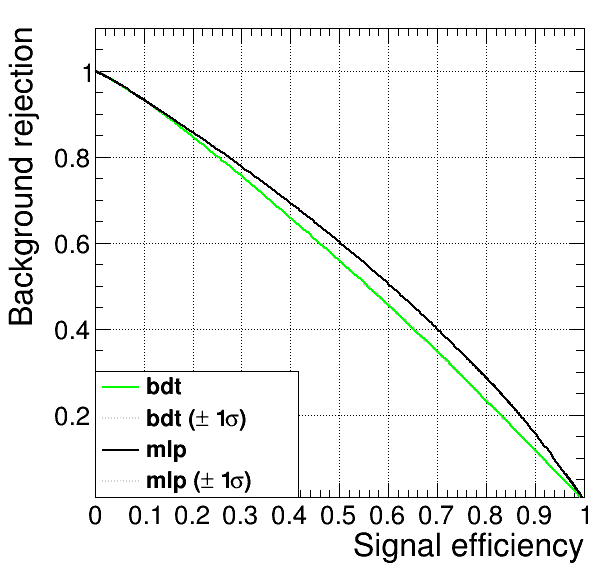
\includegraphics[width=0.5\textwidth]{figures/MVA/select1/config3/FOM_selection1_nL10_nT1000_mD5_nC50.png}
	\caption{BDT-, MLP-distribution and ROC curve for variables from selection 1 with configuration 3}
	 \label{fig:ROC_s1_config3}	
	\end{figure}

	
	\begin{figure}[H]
	\centering
	\begin{minipage}{.5\textwidth}
	  \centering
	  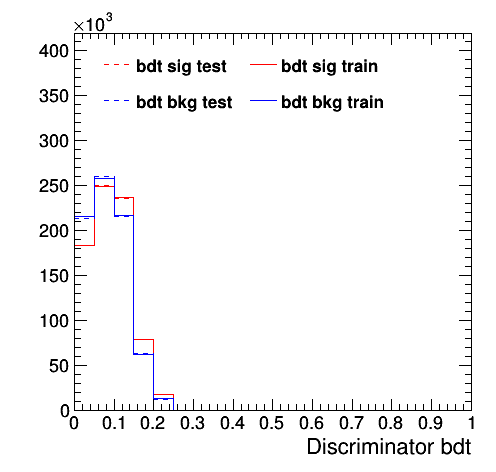
\includegraphics[width=0.75\linewidth]{figures/MVA/select2/config1/discriminator_bdt.png}
	  %\captionof{figure}{BDT distribution for selection 2 variables with configuration 1}
	  \label{fig:distr_s2_config1_bdt}
	\end{minipage}%
	\begin{minipage}{.5\textwidth}
	  \centering
	  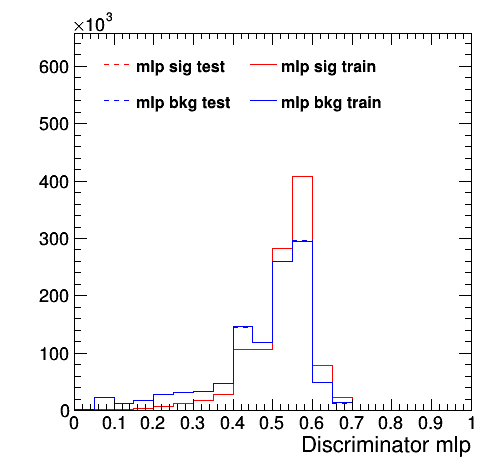
\includegraphics[width=0.75\linewidth]{figures/MVA/select2/config1/discriminator_mlp.png}
	  %\captionof{figure}{MLP distribution for selection 2 variables with configuration 1}
	  \label{fig:distr_s2_config1_mlp}
	\end{minipage}
	\centering
	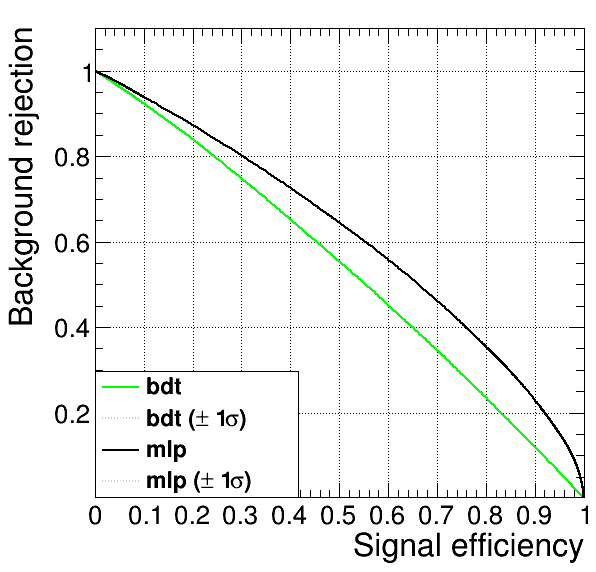
\includegraphics[width=0.5\textwidth]{figures/MVA/select2/config1/FOM_selection2_nL5_nT400_mD1_nC10.png}
	\caption{BDT-, MLP-distribution and ROC curve for variables from selection 2 with configuration 1}
	 \label{fig:ROC_s2_config1}
	\end{figure}
	
	\begin{figure}[H]
	\centering
	\begin{minipage}{.5\textwidth}
	  \centering
	  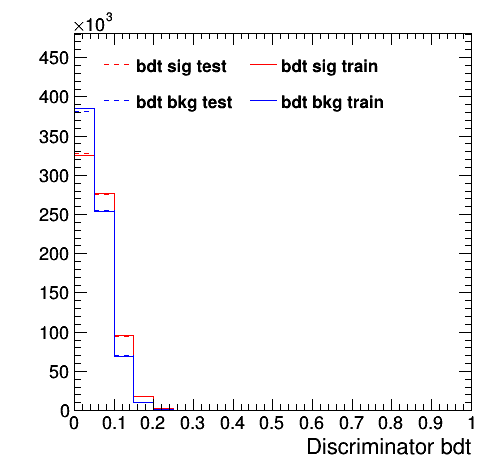
\includegraphics[width=0.75\linewidth]{figures/MVA/select2/config2/discriminator_bdt.png}
	  %\captionof{figure}{BDT distribution for selection 2 variables with configuration 2}
	  \label{fig:distr_s2_config2_bdt}
	\end{minipage}%
	\begin{minipage}{.5\textwidth}
	  \centering
	  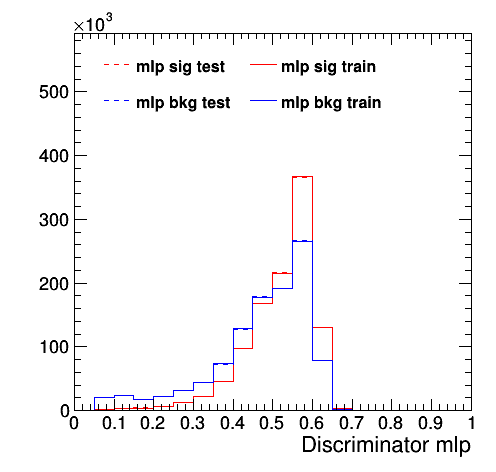
\includegraphics[width=0.75\linewidth]{figures/MVA/select2/config2/discriminator_mlp.png}
	  %\captionof{figure}{MLP distribution for selection 2 variables with configuration 2}
	  \label{fig:distr_s2_config2_mlp}
	\end{minipage}
	\centering
	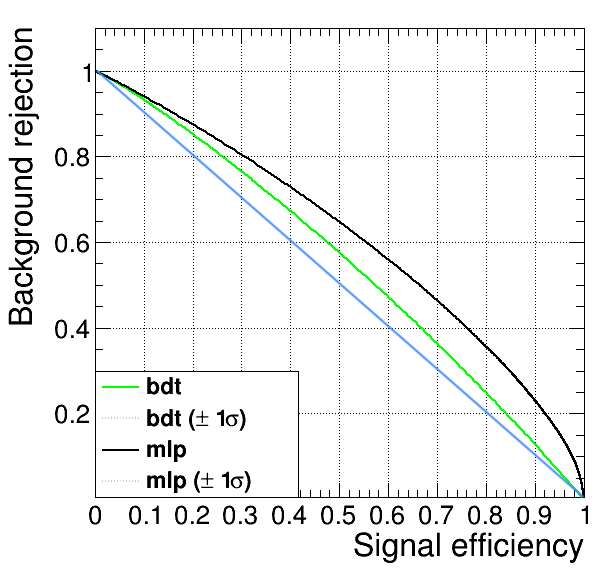
\includegraphics[width=0.5\textwidth]{figures/MVA/select2/config2/FOM_selection2_nL7_nT800_mD3_nC20.png}
	\caption{BDT-, MLP-distribution and ROC curve for variables from selection 2 with configuration 2}
	 \label{fig:ROC_s2_config2}	
	\end{figure}
	
	\begin{figure}[H]
	\centering
	\begin{minipage}{.5\textwidth}
	  \centering
	  \includegraphics[width=0.75\linewidth]{figures/MVA/select2/config3/discriminator_bdt.png}
	  %\captionof{figure}{BDT distribution for selection 2 variables with configuration 3}
	  \label{fig:distr_s2_config3_bdt}
	\end{minipage}%
	\begin{minipage}{.5\textwidth}
	  \centering
	  \includegraphics[width=0.75\linewidth]{figures/MVA/select2/config3/discriminator_mlp.png}
	  %\captionof{figure}{MLP distribution for selection 2 variables with configuration 3}
	  \label{fig:distr_s2_config3_mlp}
	\end{minipage}
	\centering
	\includegraphics[width=0.5\textwidth]{figures/MVA/select2/config3/FOM_selection2_nL10_nT1000_mD5_nC50.png}
	\caption{BDT-, MLP-distribution and ROC curve for variables from selection 2 with configuration 3}
	 \label{fig:ROC_s2_config3}	
	\end{figure}
	
	
	\begin{figure}[H]
	\centering
	\begin{minipage}{.5\textwidth}
	  \centering
	  \includegraphics[width=0.75\linewidth]{figures/MVA/select3/config1/discriminator_bdt.png}
	  %\captionof{figure}{BDT distribution for selection 3 variables with configuration 1}
	  \label{fig:distr_s3_config1_bdt}
	\end{minipage}%
	\begin{minipage}{.5\textwidth}
	  \centering
	  \includegraphics[width=0.75\linewidth]{figures/MVA/select3/config1/discriminator_mlp.png}
	  %\captionof{figure}{MLP distribution for selection 3 variables with configuration 1}
	  \label{fig:distr_s3_config1_mlp}
	\end{minipage}
	\centering
	\includegraphics[width=0.5\textwidth]{figures/MVA/select3/config1/FOM_selection3_nL5_nT400_mD1_nC10.png}
	\caption{BDT-, MLP-distribution and ROC curve for variables from selection 3 with configuration 1}
	 \label{fig:ROC_s3_config1}
	\end{figure}
	
	\begin{figure}[H]
	\centering
	\begin{minipage}{.5\textwidth}
	  \centering
	  \includegraphics[width=0.75\linewidth]{figures/MVA/select3/config2/discriminator_bdt.png}
	  %\captionof{figure}{BDT distribution for selection 3 variables with configuration 2}
	  \label{fig:distr_s3_config2_bdt}
	\end{minipage}%
	\begin{minipage}{.5\textwidth}
	  \centering
	  \includegraphics[width=0.75\linewidth]{figures/MVA/select3/config2/discriminator_mlp.png}
	  %\captionof{figure}{MLP distribution for selection 3 variables with configuration 2}
	  \label{fig:distr_s3_config2_mlp}
	\end{minipage}
	\centering
	\includegraphics[width=0.5\textwidth]{figures/MVA/select3/config2/FOM_selection3_nL7_nT800_mD3_nC20.png}
	\caption{BDT-, MLP-distribution and ROC curve for variables from selection 3 with configuration 2}
	 \label{fig:ROC_s3_config2}	
	\end{figure}
	
	\begin{figure}[H]
	\centering
	\begin{minipage}{.5\textwidth}
	  \centering
	  \includegraphics[width=0.75\linewidth]{figures/MVA/select3/config3/discriminator_bdt.png}
	  %\captionof{figure}{BDT distribution for selection 3 variables with configuration 3}
	  \label{fig:distr_s3_config3_bdt}
	\end{minipage}%
	\begin{minipage}{.5\textwidth}
	  \centering
	  \includegraphics[width=0.75\linewidth]{figures/MVA/select3/config3/discriminator_mlp.png}
	  %\captionof{figure}{MLP distribution for selection 3 variables with configuration 3}
	  \label{fig:distr_s3_config3_mlp}
	\end{minipage}
	\centering
	\includegraphics[width=0.5\textwidth]{figures/MVA/select3/config3/FOM_selection3_nL10_nT1000_mD5_nC50.png}
	\caption{BDT-, MLP-distribution and ROC curve for variables from selection 3 with configuration 3}
	 \label{fig:ROC_s3_config3}	
	\end{figure}
				
\section{Conclusion}
It is very difficult to differentiate between $t\overline{t}\gamma$ and $t\overline{t}$ events because they show very similiar behaviour in the signal region. Nevertheless, a slight improvement was possible by training a MVA with relevant variables. Especially photon variables provide a bigger improvement. MLPs show a better performance than BDTs, which suggests the selection of this type of model.

\section{Bibliography}

\section{List of figures}

\section{Appendix}
	\subsection{Full list of variables with almost identical distributions}
	\label{sec:annex-identical}
	\begin{figure}[H]
	\centering
	\begin{minipage}{.5\textwidth}
	  \centering
	  \includegraphics[width=0.75\linewidth]{figures/Notused/Bj0_eta.png}
	  \captionof{figure}{Bj0\_eta}
	\end{minipage}%
	\begin{minipage}{.5\textwidth}
	  \centering
	  \includegraphics[width=0.75\linewidth]{figures/Notused/Bj0_phi.png}
	  \captionof{figure}{Bj0\_phi}
	\end{minipage}
	\end{figure}
	
	\begin{figure}[H]
	\centering
	\begin{minipage}{.5\textwidth}
	  \centering
	  \includegraphics[width=0.75\linewidth]{figures/Notused/Bj0_pt.png}
	  \captionof{figure}{Bj0\_pt}
	\end{minipage}%
	\begin{minipage}{.5\textwidth}
	  \centering
	  \includegraphics[width=0.75\linewidth]{figures/Notused/Bj1_eta.png}
	  \captionof{figure}{Bj1\_eta}
	\end{minipage}
	\end{figure}
	
	\begin{figure}[H]
	\centering
	\begin{minipage}{.5\textwidth}
	  \centering
	  \includegraphics[width=0.75\linewidth]{figures/Notused/Bj1_phi.png}
	  \captionof{figure}{Bj1\_phi}
	\end{minipage}%
	\begin{minipage}{.5\textwidth}
	  \centering
	  \includegraphics[width=0.75\linewidth]{figures/Notused/Bj1_pt.png}
	  \captionof{figure}{Bj1\_pt}
	\end{minipage}
	\end{figure}
	
	\begin{figure}[H]
	\centering
	\begin{minipage}{.5\textwidth}
	  \centering
	  \includegraphics[width=0.75\linewidth]{figures/Notused/JetGood0_btagDeepB.png}
	  \captionof{figure}{JetGood0\_btagDeepB}
	\end{minipage}%
	\begin{minipage}{.5\textwidth}
	  \centering
	  \includegraphics[width=0.75\linewidth]{figures/Notused/JetGood0_chEmEF.png}
	  \captionof{figure}{JetGood0\_chEmEF}
	\end{minipage}
	\end{figure}
	
	\begin{figure}[H]
	\centering
	\begin{minipage}{.5\textwidth}
	  \centering
	  \includegraphics[width=0.75\linewidth]{figures/Notused/JetGood0_chHEF.png}
	  \captionof{figure}{JetGood0\_chHEF}
	\end{minipage}%
	\begin{minipage}{.5\textwidth}
	  \centering
	  \includegraphics[width=0.75\linewidth]{figures/Notused/JetGood0_neEmEF.png}
	  \captionof{figure}{JetGood0\_neEmEF}
	\end{minipage}
	\end{figure}
	
	\begin{figure}[H]
	\centering
	\begin{minipage}{.5\textwidth}
	  \centering
	  \includegraphics[width=0.75\linewidth]{figures/Notused/JetGood0_neHEF.png}
	  \captionof{figure}{JetGood0\_neHEF}
	\end{minipage}%
	\begin{minipage}{.5\textwidth}
	  \centering
	  \includegraphics[width=0.75\linewidth]{figures/Notused/JetGood1_btagDeepB.png}
	  \captionof{figure}{JetGood1\_btagDeepB}
	\end{minipage}
	\end{figure}
	
	\begin{figure}[H]
	\centering
	\begin{minipage}{.5\textwidth}
	  \centering
	  \includegraphics[width=0.75\linewidth]{figures/Notused/JetGood1_eta.png}
	  \captionof{figure}{JetGood1\_eta}
	\end{minipage}%
	\begin{minipage}{.5\textwidth}
	  \centering
	  \includegraphics[width=0.75\linewidth]{figures/Notused/JetGood1_phi.png}
	  \captionof{figure}{JetGood1\_phi}
	\end{minipage}
	\end{figure}
	
	\begin{figure}[H]
	\centering
	\begin{minipage}{.5\textwidth}
	  \centering
	  \includegraphics[width=0.75\linewidth]{figures/Notused/JetGood1_pt.png}
	  \captionof{figure}{JetGood1\_pt}
	\end{minipage}%
	\begin{minipage}{.5\textwidth}
	  \centering
	  \includegraphics[width=0.75\linewidth]{figures/Notused/LeptonTight0__phi.png}
	  \captionof{figure}{LeptonTight0\_phi}
	\end{minipage}
	\end{figure}
	
	\begin{figure}[H]
	\centering
	\begin{minipage}{.5\textwidth}
	  \centering
	  \includegraphics[width=0.75\linewidth]{figures/Notused/LeptonTight0_eta.png}
	  \captionof{figure}{LeptonTight0\_eta}
	\end{minipage}%
	\begin{minipage}{.5\textwidth}
	  \centering
	  \includegraphics[width=0.75\linewidth]{figures/Notused/LeptonTight0_pfRelIso03_all.png}
	  \captionof{figure}{LeptonTight0\_pfRelIso03\_all}
	\end{minipage}
	\end{figure}
	
	\begin{figure}[H]
	\centering
	\begin{minipage}{.5\textwidth}
	  \centering
	  \includegraphics[width=0.75\linewidth]{figures/Notused/LeptonTight0_pfRelIso03_chg.png}
	  \captionof{figure}{LeptonTight0\_pfRelIso03\_chg}
	\end{minipage}%
	\begin{minipage}{.5\textwidth}
	  \centering
	  \includegraphics[width=0.75\linewidth]{figures/Notused/LeptonTight0_pfRelIso03_ne.png}
	  \captionof{figure}{LeptonTight0\_pfRelIso03\_ne}
	\end{minipage}
	\end{figure}
	
	\begin{figure}[H]
	\centering
	\begin{minipage}{.5\textwidth}
	  \centering
	  \includegraphics[width=0.75\linewidth]{figures/Notused/LeptonTight0_pt.png}
	  \captionof{figure}{LeptonTight0\_pt}
	\end{minipage}%
	\begin{minipage}{.5\textwidth}
	  \centering
	  \includegraphics[width=0.75\linewidth]{figures/Notused/nElectronTight.png}
	  \captionof{figure}{nElectronTight}
	\end{minipage}
	\end{figure}
	
	\begin{figure}[H]
	\centering
	\begin{minipage}{.5\textwidth}
	  \centering
	  \includegraphics[width=0.75\linewidth]{figures/Notused/nHighPTPhotons.png}
	  \captionof{figure}{nHighPTPhotons}
	\end{minipage}%
	\begin{minipage}{.5\textwidth}
	  \centering
	  \includegraphics[width=0.75\linewidth]{figures/Notused/nJet.png}
	  \captionof{figure}{nJet}
	\end{minipage}
	\end{figure}
	
	\begin{figure}[H]
	\centering
	\begin{minipage}{.5\textwidth}
	  \centering
	  \includegraphics[width=0.75\linewidth]{figures/Notused/nLeptonTight.png}
	  \captionof{figure}{nLeptonTight}
	\end{minipage}%
	\begin{minipage}{.5\textwidth}
	  \centering
	  \includegraphics[width=0.75\linewidth]{figures/Notused/nMuonTight.png}
	  \captionof{figure}{nMuonTight}
	\end{minipage}
	\end{figure}
	
	\begin{figure}[H]
		\begin{center}
		\includegraphics[width=0.38\textwidth]{figures/Notused/nPhotonGood.png}
		\caption{nPhotonGood}
		\end{center}
	\end{figure}

	\subsection{Excluded variables}
	\label{sec:annex-excluded}
	\begin{figure}[H]
	\centering
	\begin{minipage}{.5\textwidth}
	  \centering
	  \includegraphics[width=0.75\linewidth]{figures/Notused/PhotonGood0_pfRelIso03_chg.png}
	  \captionof{figure}{PhotonGood0\_pfRelIso03\_chg}
	\end{minipage}%
	\begin{minipage}{.5\textwidth}
	  \centering
	  \includegraphics[width=0.75\linewidth]{figures/Notused/PhotonGood0_pfRelIso03_ne.png}
	  \captionof{figure}{PhotonGood0\_pfRelIso03\_ne}
	\end{minipage}
	\end{figure}
	
	\begin{figure}[H]
		\begin{center}
		\includegraphics[width=0.38\textwidth]{figures/Notused/tightLeptonJetdR.png}
		\caption{tightLeptonJetdR}
		\end{center}
	\end{figure}
	
\end{document}
